\documentclass[aps,prb,preprint,notitlepage]{revtex4-2}

\usepackage{graphicx}% Include figure files
\usepackage{dcolumn}% Align table columns on decimal point
\usepackage{bm}% bold math
\usepackage{hyperref}% add hypertext capabilities

\begin{document}

\title{Superconductivity, magnetism and directional plasmonic modes in 
two-dimensional penta-bipyramid boron allotropes} 
\author{L.\ Niu$^{1}$,  O.\ J.\ Conquest$^{1,*}$,  H.\ Ma$^{1}$, C.\ Verdi$^{1,2}$, and C.\ Stampfl$^{1,*}$}
\affiliation{$^{1}$School of Physics, The University of Sydney,  NSW 2006, Australia\\
$^{2}$ School of Mathematics and Physics, The University of Queensland, QLD 4072, Australia}
\begin{abstract}
	Bulk orthorhombic boron (o-B14) is an intriguing, recently predicted,
	three-dimensional (3D) boron allotrope. 
	Its structure is characterized by edge-sharing pentagonal bipyramids, with 
	diverse bond lengths. 
	These structural motifs facilitate the formation of unusual seven-centre-two-electron $\pi$-bonds, predicted for the first time in 
	3D boron allotropes. 
	The presence of these bonds highlights the complexity and versatility of boron chemistry under ambient conditions. Moreover, this material
	is predicted to be a superconductor with a critical temperature 
	$T_c$
	of 29.1 K [Phys.Chem.Chem.Phys. {\bf 25}, 15400 (2023)].
In the present work, we explore the electronic and optical properties of bulk o-B14 
and its monolayer and bilayer forms, 
including hydrogen termination, 
	using first-principles calculations. 
	These two-dimensional structures are predicted to be dynamically 
	stable and to exhibit a remarkable variety of electronic behaviour including
	semiconductivity with a band-gap of 0.67~eV (bilayer), 
	superconductivity with a $T_c$ of 24.3 K 
	(H-terminated bilayer) and magnetism (monolayer).
	The plasmonic and optical responses exhibit anisotropic behaviour 
	driven by the directional 
	bonding network, as well as absorption in the visible region of the 
	spectrum, which suggest promising opportunities for applications in
	advanced optoelectronic, plasmonic  and quantum devices.
\end{abstract}

\pacs{}

\maketitle
\def\figurename{FIG.}\def\tablename{TABLE}


\section{Introduction} Elemental boron possesses a unique combination of light weight, exceptional hardness, and thermal and chemical stability. 
Due to these properties, it has potential for 
high technology applications such as catalysis, sensors, energy storage, 
piezoelectrics, and nanodevices~\cite{ranjan2024properties}.
Boron exists in multiple allotropes with complex crystal structures arising from its electron-deficient bonding and small atomic size. The most well-characterized and stable crystalline forms are $\alpha$-rhombohedral boron ($\alpha$-B, 12 atoms per unit cell), $\beta$-rhombohedral boron ($\beta$-B, 105-108 atoms per unit cell) \cite{widom2008symmetry}  and $\gamma$-orthorhombic boron ($\gamma$-B, 28 atoms per unit cell) \cite{an2016new}. $\alpha$-B consists of B$_{12}$ icosahedra building blocks and forms 
at low temperature, while $\beta$-B has the same structure, but also includes
interstitial B atoms. It forms at room temperature and is the most stable structure.  $\gamma$-B is also composed of B$_{12}$ icosahedra units and forms at high pressure and 
temperature. 
The structures are predominantly characterized by covalent bonding, 
but the electron deficiency of boron gives rise to multi-centre bonding (e.g., 
3-center-2-electron bonds). 
Additionally, boron-rich compounds exhibit promising 
semiconducting and thermoelectric properties, with 
potential use in next-generation electronics and energy-harvesting devices.
\\
Generally, the superconducting critical temperature ($T_c$) of elemental superconductors is relatively low at ambient pressure, e.g. Nb has a $T_c$ of 
about 9 K. Under high pressure the $T_c$ can be significantly increased compared to at ambient pressure, but high pressure hinders experimental studies and practical applications, thus it is of high priority to explore elemental 
superconductors with high a $T_c$ under low or ambient pressure.
Interestingly,  superconductivity with a $T_c$ of 35 K has been reported 
in a three-dimensional (3D) kagome-like boron allotrope under 7 
GPa on the basis of {\em ab initio} 
calculations~\cite{ouyang2025superconductivity}, while earlier work predicts
a $T_c$ exceeding 15 K in 3D  boron allotropes~\cite{zhang2020superconducting}.

Boron can also form isolated clusters which exhibit many intriguing properties including fluxionality \cite{pan2019fluxional}, that is
the ability to
undergo continuous structural rearrangements without breaking chemical 
bonds in a way that permanently alters the system.
Recent studies have focused on two-dimensional (2D) forms of boron, 
including monolayer borophene, where many different structures have been observed as explained in recent review papers: Wang {\em et al.} \cite{ wang2024borophene} have summarized the synthesis and properties of borophene while Mishra {\em et al. }
\cite{mishra2024borophene}
 have reviewed the potential of borophene in various technological fields such as batteries, supercapacitors, fuel cells and the associated synthesis techniques. Other recent reviews of borophene focus on experiment \cite{mohanty2023review,yang2023borophenes,kumar2024rise, xie2020two}, and provide a survey of structures starting from the bulk allotropes, boron clusters, potential building blocks for 2D boron crystals and 2D few-layered boron sheets ~\cite{sun2017two}.
Being a light 2D material, and also possessing good flexibility, 
endows it with potential applications in flexible and wearable devices, 
in biomedicines, and 
biosensors~\cite{mozvashi2021mechanical,zhang2017elasticity}.

From the theoretical side, 2D boron has also attracted significant recent interest due to its complex electronic structure which can give rise to predicted semiconducting 
behaviour \cite{qureshi2024bilayer} including in twisted bilayer borophene \cite{jin2022tuning}, superconductivity \cite{gao2017prediction,han2023superconducting}, magnetism \cite{zhu2019magnetic}  and topological states
\cite{wang2025second,rakshit2025exploring,wang2019serendipity}.  
Furthermore, the $\beta_{12}$ sheet has been found to host gapless Dirac cones
~\cite{feng2017dirac} and a bilayer kagome structure has been predicted to host
multiple van Hove singularities~\cite{gao2024bilayer}.
Half-metallic ferromagnetism has also been reported in a 2D kagome lattice 
composed of a triangular arrangement of boron atoms within 
triangles~\cite{kim2017boron}.



Synthesizing borophene is notably challenging due to several intrinsic and extrinsic factors. Unlike graphene, borophene lacks a naturally occurring layered bulk counterpart, which eliminates the possibility of exfoliation-based synthesis. Its high chemical reactivity, especially with oxygen and moisture, makes it unstable under ambient conditions, requiring 
ultra-high vacuum (UHV) environments for fabrication and handling. These factors collectively make the reproducible and scalable synthesis of monolayer 
borophene a significant materials science hurdle.
To overcome the challenges of synthesizing monolayer borophene, researchers have focused on carefully controlled epitaxial growth techniques such as molecular beam epitaxy (MBE) on inert metal substrates \cite{chen2022synthesis}. 
Another study has achieved growth of $\beta_{12}$- and $\alpha$-sheets of 
borophene on Ag(111) by direct evaporation of a pure boron source in an e-beam evaporator~\cite{zhong2017metastable}.

Substrates stabilize the 2D structure of borophene during growth by promoting specific polymorphs through surface templating. Maintaining 
UHV conditions during synthesis helps prevent oxidation and contamination.
Another strategy to enhance the stability is to use hydrogen termination,   which passivates the highly reactive surface boron atoms. 
This passivation can reduce the tendency to oxidize or react with 
ambient species, thereby improving chemical stability in air. Moreover, hydrogen termination can modify the electronic properties, potentially opening a band-gap or altering metallic behaviour, which may be advantageous for specific 
applications \cite{hou2020ultrastable,li2021synthesis}. Large-scale 
synthesis of freestanding atomic sheets of borophene has been reported through a 
novel liquid-phase exfoliation approach, where electron microscopy 
confirmed the presence of the $\beta_{12}$ and $\chi_{3}$ phases, as well
as their intermediate phases \cite{ranjan2019freestanding}.

 Different from the flat borophenes, a novel highly stable 2D boron structure has been recently predicted on the basis of {\em ab initio} calculations. It is
 composed of  B$_{12}$ clusters 
linked by single B-B bonds and is a 
narrow band-gap semiconductor \cite{zhang2023novel}.
The optical properties of 2D allotropes have also been investigated, where
it has been reported that the plasmon frequencies reach the near infrared,
and even visible regions, making borophene among the first materials with 2D plasmons
at such high energies without
doping~\cite{huang2017two}.

Recently, a bulk orthorhombic boron allotrope (o-B14) with
interesting 
properties was predicted~\cite{han2023superconducting}. 
Its structure is characterized 
by edge-sharing pentagonal bipyramids with varying B-B bond lengths
	ranging from 1.644 to 1.966 Å. 
These structural
motifs facilitate the formation of peculiar seven-centre-two-electron 
$\pi$-bonds,  which are found for the first time in 3D 
boron allotropes. 
Remarkably, this material is
predicted to be a superconductor with a transition temperature of 29.1 K.

This orthorhombic o-B14 structure is a particularly promising candidate 
for further investigation because it introduces the pentagonal 
B$_7$ bipyramidal motif as a fundamental structural unit in crystalline 
boron, which differs markedly from the B$_{12}$ icosahedral units that 
dominate most known boron phases. This unusual topology leads to highly 
delocalized multicentre bonding, including the predicted seven-centre 
two-electron $\pi$ bonds, suggesting that the electronic structure may 
host unconventional features such as anisotropic transport, unusual phonon 
behaviour, and potentially strong electron-phonon coupling. 
Since the phase is predicted to be energetically competitive and 
dynamically stable at ambient pressure, {\em ab initio} studies of 
its electronic band structure, phonon spectrum, and superconducting 
properties, as well as for exploring how the unique bipyramidal 
building blocks influence the broader physics of electron-deficient 
boron networks would be valuable. Moreover, the question also arises 
as to whether it may be stable in 2D form where 
the interlayer connectivity consists of just single B-B bonds.

In the present work we use density-functional theory
(DFT) calculations to investigate the electronic and optical
properties of bulk o-B14 and its mono- and bilayers. 
Hydrogen termination of the 2D structures is also considered. 
Interestingly, bilayer o-B14 is found to be a semiconductor with a band-gap of around
0.69~eV as calculated using the HSE06 hybrid functional.
The H-terminated bilayer, however, is predicted to be superconducting with 
a $T_c$ of 24.3 K, while monolayer o-B14 is found to be magnetic.
The optical properties reveal distinctive anisotropic behaviors and the existence
of plasmons in the near to mid-infrared range for in-plane excitation as
well as the ultra-violet energy range for out-of-plane,
broadening the potential of boron for applications 
in optoelectronics, plasmonics and catalysis.

The paper is organised as follows: in Section 2 the computation  methods are
presented, followed by the results and discussion in Section 3. Herein 
we describe the electronic, superconducting and optical properties.
This is followed by the  conclusion in Section 4.



\section{Computation Methods}

The DFT calculations are performed using the  
Vienna Ab initio Simulation Package (VASP) 
\cite{kresse1993ab,kresse1996efficiency,kresse1994ef,kresse1994ab}. The projector 
augmented wave (PAW) method pseudopotentials are used to 
describe the electron-ion interactions \cite{kresse1999ultrasoft}. 
The generalized gradient approximation (GGA) of Perdew-Burke-Ernzerhof (PBE) 
for the exchange-correlation functional~\cite{PBE-1996} is employed along with the 
Becke-Johnson damped D3(BJ) dispersion correction to account for long-range 
van der Waals (vdW) interactions~\cite{D3BJ2005,D3BJ2010,D3BJ2011}. 
For bulk o-B14, a $\Gamma$-centered {\bf k}-point 
mesh of $34 \times 48 \times 31$ is used with a plane-wave energy cutoff of 
$600\text{ eV}$. 
The electronic convergence criterion is set to $10^{-6}$ eV and the structures
are relaxed until all forces on each atom are below 0.01 eV/$\mathring{\text{A}}$. 
For the 2D systems, a vacuum region of $\approx$22~\AA, is included and 
a {\bf k}-point
mesh of $20 \times 18 \times 1$ is used.
Convergence tests show that these settings yieild accurate results as 
shown in Figs. S1-S3 of the Supplementary Information (SI).  


For selected calculations we also use the screened hybrid exchange-correlation 
functional of Heyd, Scuseria, and Ernzerhof (HSE06) which gives more 
accurate band-gap energies \cite{PBE_Vs_HSE06_2021, HSE06_2003, HSE06_2006}. 
All figures show results obtained using the PBE functional unless explicitly stated otherwise.
For the density-of-states (DOS) calculations for bulk o-B14, we 
use a $\Gamma$-centered {\bf k}-point 
mesh of $20 \times 28 \times 18$ and for the 2D systems, 
$20 \times 18 \times 1$,  with smearing at the Fermi level 
calculated with the Gaussian method and a broadening value of $0.1$ eV. 

The adsorption energy per atom, $E_{\mathrm{ad}}$, of hydrogen atoms on the surface is 
calculated using Eq.~(\ref{eq-be}), 
\begin{equation}
	E_{\mathrm{ad}} = (E_{\mathrm{H/B}} - E_{\mathrm{B}} - E_{\mathrm{H}})/n_{\rm H}
    \label{eq-be}
\end{equation}
where $E_{\mathrm{H/B}}$ is the total energy of the adsorption system, $E_{\mathrm{B}}$ is the total energy of the 2D 
pristine boron structure and $E_{\mathrm{H}}$ is the total energy of a 
hydrogen atom in the H$_{2}$ molecule, and $n_{\rm H}$ is the number
of H atoms in the unit cell.   

The cohesive energy per atom of the boron systems is calculated as,
\begin{equation}
	E_{\mathrm{c}} = (E_{\mathrm{B-struc}} - nE_{\mathrm{B-atom}})/n_{\rm B} 
    \label{eqn:binding_energy}
\end{equation}
where $E_{\mathrm{B-struc}}$ is the total energy of the boron structure of interest and
$E_{\mathrm{B-atom}}$ is the total energy of a free boron atom calculated in a large
supercell. $n_{\rm B}$ is the number of boron atoms in the unit cell of the structure.

The charge density difference, $\Delta \rho(\bf{r})$, for hydrogen adsorption on the surface is calculated using Eq.~(\ref{eqn:charge_difference}):


\begin{equation}
    \Delta \rho (\bf{r}) = \rho_{\mathrm{H/B}}(\bf{r}) - \rho_{\mathrm{B}}(\bf{r}) - \rho_{\mathrm{H}}(\bf{r})
    \label{eqn:charge_difference}
\end{equation}
The term
$\rho_{\mathrm{H/B}}(\bf{r})$ is the total charge density of the adsorbed system and $\rho_{\mathrm{B}}(\bf{r})$ and $\rho_{\mathrm{H}}(\bf{r})$  are the total charge densities of the clean boron structure and the hydrogen atom, respectively.    

The superconducting behavior of o-B14 is investigated systematically in 
three structural phases: bulk, monolayer, and hydrogen-terminated bilayer. 
Calculations are carried out 
using the PBE~\cite{PBE-1996} 
formulation of the generalized gradient approximation, as provided in 
Quantum ESPRESSO~\cite{giannozzi2009quantum}.  
Norm-conserving pseudopotentials and a kinetic 
energy cutoff of 45 Ry are chosen~\cite{hamann2013optimized}, and a vacuum spacing of 15~\AA\,
is added for the 2D systems to suppress spurious periodic 
interactions. Monkhorst-Pack {\bf k}-meshes of 9$\times$12$\times$8 for the bulk, 
10$\times$10$\times$1 for the monolayer, and 9$\times$9$\times$1 for the 
bilayer are employed to sample the Brillouin zone~\cite{methfessel1989high}. The phonon 
dispersions are calculated on {\bf q}-point grids of 
3$\times$4$\times$3, 5$\times$5$\times$1, and 3$\times$3$\times$1, 
respectively~\cite{baroni2001phonons}. Atomic positions and lattice parameters are 
relaxed until residual forces are below 1$\times 10^{-5}$ Ry/bohr (2.6$\times 10^{-4}$ eV/\AA). 
Maximally localized Wannier functions are constructed in Wannier90 by 
initializing projections on B $s$ and $p$ orbitals~\cite{pizzi2020wannier90}. Uniform 
{\bf k}-meshes of 6$\times$8$\times$6 (bulk) and 6$\times$6$\times$1 
(monolayer and bilayer) are used in Wannier interpolation. Superconductivity 
is subsequently analyzed through 
EPW~\cite{giannozzi2009quantum,giannozzi2020quantum,giannozzi2017advanced},
which is employed to 
evaluate electron-phonon coupling strength and estimate Allen-Dynes transition 
temperatures ($T_c$)~\cite{margine2013anisotropic}. 
The superconducting properties are also obtained by solving the fully anisotropic Migdal-Eliashberg equations~\cite{bardeen1955electron,giustino2017electron,margine2013anisotropic}, as implemented in the EPW code.
The Morel-Anderson pseudopotential 
$\mu^{*}$ was chosen to be 0.13, consistent with the 
typical semi-empirical range of 0.10 - 0.16 used in Migdal-Eliashberg 
calculations for light-element and $sp$-bonded superconductors~\cite{allen-dynes} and with the value adopted in the literature for boron-based 2D superconductors~\cite{zhao2019two}. With this choice,
the calculated electron-phonon coupling strengths 
$(\lambda)$  and $T_c$ indicate clear dimensionality effects as discussed 
in Sec. IIIC.


For the calculation of the optical properties within VASP, in particular, the 
frequency-dependent dielectric function, the {\bf k}-point meshes 
of ($20\times28\times18$) and ($20\times18\times1)$ are 
found to yield converged results (cf. Fig. S4) for the bulk and 2D systems, respectively.
A convergence check for the number of unoccupied bands to 
include 
in the calculation of the dielectric function was also performed. 
Figure S5 shows the results 
for bulk o-B14. It can be seen that $128$ bands yield 
well-converged results and hereafter this value is used for all systems.

The complex frequency-dependent dielectric function, $\epsilon(\omega)$, 
is given by $\epsilon(\omega) = \epsilon_{1}(\omega) + i\epsilon_{2}(\omega)$, where $\epsilon_{1}(\omega)$ 
and $\epsilon_{2}(\omega)$ are the real and imaginary parts, respectively, 
and $\omega$ is the frequency in eV.

The imaginary part of the dielectric function, $\epsilon_{2}(\omega)$, is calculated as:
\begin{displaymath}
    \epsilon_{2}(\omega) = \mathrm{Im} \ \epsilon_{\boldsymbol{\alpha} \boldsymbol{\beta}} (\omega) = \frac{4\pi^{2}e^{2}}{\Omega} \lim_{q\rightarrow0} \frac{1}{q^2} \sum_{c,v,\mathbf{k}} 2\omega_{\mathbf{k}} \delta(E_{c\mathbf{k}}-E_{v\mathbf{k}}-\omega) 
\end{displaymath}
\begin{equation}
	\times \langle {u_{c\mathbf{k}+\mathbf{e}_{\boldsymbol{\alpha}} q}
	|u_{v\mathbf{k}}}\rangle \langle {u_{v\mathbf{k}}|u_{c\mathbf{k}+
	\mathbf{e}_{\boldsymbol{\beta}} q}}\rangle  
    \label{eqn:dielectric_im}
\end{equation}
where $\mathbf{k}$ is the electron wavevector, $\omega_{\mathbf{k}}$ is the $\mathbf{k}$-point weight, $q$ is the Bloch vector for the incident wave and $\Omega$ is the unit cell volume~\cite{Dielectric_textbook,VASP_Dielectric_2006}. 
Here $v$ and $c$ are the valence and conduction band indices, respectively. The $u_{v\mathbf{k}/c\mathbf{k}}$ terms are the cell periodic parts of the orbitals and $\mathbf{e}_{\boldsymbol{\alpha/\beta}}$ are the unit vectors for the three Cartesian directions. $E_{c\mathbf{k}}$ is the $c^{\mathrm{th}}$ conduction band energy and $E_{v\mathbf{k}}$ is the $v^{\mathrm{th}}$ valence band~energy. 


The real part of the dielectric function is obtained by applying the 
Kramers-Kronig transformation:
\begin{equation}
    \epsilon_{1}(\omega) = \mathrm{Re} \ \epsilon_{\boldsymbol{\alpha} \boldsymbol{\beta}} (\omega) = \delta_{\boldsymbol{\alpha} \boldsymbol{\beta}} + \frac{2}{\pi}P \int_{0}^{\infty} \mathrm{d}\omega' \frac{\omega'\epsilon_{2}(\omega')}{\omega'^{2}-\omega^{2}+i\eta}
    \label{eqn:dielectric_real}
\end{equation}
where $P$ is the principal~value and $\eta$ (here $\eta=0.1$) is the complex 
shift.

From the dielectric function the absorption coefficient $\alpha(\omega)$, the loss function $L(\omega)$, the refractive index $n(\omega)$, the extinction coefficient $k(\omega)$ and reflectivity $R(\omega)$ can be calculated using Eqs.~1-5 of the SI.


The dielectric tensor contains the combined dielectric response 
of the 2D material and the vacuum so that the magnitude 
of $\epsilon_{1}$ and $\epsilon_{2}$ depend linearly on the vacuum thickness~\cite{Dielectric_vacuum_1,Dielectric_vacuum_2}. 
Therefore, to obtain the intrinsic dielectric function of the structures, 
the calculated dielectric functions need to be renormalized. This is performed 
using Eq.~\ref{eq-norm1} and Eq.~\ref{eq-norm2},
following Ref.~\cite{yang2021method}:


\begin{equation}
	(\epsilon_{2})_{2D} = \frac{d_{SC}}{d_{2D}}(\epsilon_{2})_{SC}
	\label{eq-norm1}
\end{equation}
\begin{equation}
	(\epsilon_{1})_{2D} = 1 + \frac{d_{SC}}{d_{2D}}((\epsilon_{1})_{SC}
	-1)
	\label{eq-norm2}
\end{equation}
In these equations, $(\epsilon_{i})_{2D}$  and
 $(\epsilon_{i})_{SC}$  $(i=1,2)$ are the dielectric functions of the studied 2D structure without the influence of the vacuum region and for the whole supercell, respectively, and $d_{SC}$ is the length of the supercell.
 The thickness ($d_{2D}$) for  the monolayer, bilayer and H-terminated bilayer is 5.897~\AA, 9.412~\AA, and 11.209~\AA, respectively. The thickness is defined in Fig. S6 of the  SI.
In the literature, this correction is often ignored in studies on 2D materials, which leads to errors in the reported dielectric functions and therefore the optical properties of the 2D materials.
It is noted that interband transitions presumably coexist with the 
plasmons forming a broad background. The coexistence of individual transitions 
and plasmons in the same energy range leads to a coupling 
of the two types of excitations, and hence finite plasmon 
lifetimes as  well as interband transitions \cite{li2017first}. 


\section{Results and Discussion}

\subsection{Bulk o-B14: Atomic structure and electronic properties}

The structural and electronic properties of bulk o-B14 are investigated first. 
The atomic structure is shown in Fig.~\ref{fig-bulk}a.  
This allotrope of boron (along with several others) has been predicted, on the basis of first-principles calculations, to be dynamically and thermodynamically stable~\cite{han2023superconducting}. 
The structural properties are listed in Table \ref{tab-1}. 
Following Ref.~\cite{han2023superconducting}, the 
boron atoms in the unit cell are assigned to  three groups as 
indicated by the circles in Fig.~\ref{fig-bulk}b and sketched in Fig.~\ref{fig-bulk}d.  
This was done using 
the approach of solid state adaptive natural density partitioning 
(SSAdNDP)~\cite{zubarev2008developing} to analyse the multicenter bonding. This method is 
an attempt to combine the ideas of Lewis theory and aromaticity. 
It was found that 
aside from the four normal 2-centre -- 2-electron and the sixteen 3-center -- 2-electron B-B $\sigma$ bonds, there are unusual 
7-center -- 2-electron $\pi$ bonds~\cite{han2023superconducting}.

The band structure, shown in Fig.~\ref{fig-bs-bulk} (upper), 
exhibits metallic behavior with three bands crossing the Fermi level. 
These bands include steep bands promoting high electron velocities and flat 
bands near the Fermi level, enhancing the density-of-states (DOS) and favoring 
electronic interactions. Such electronic features suggest the potential for 
unique transport and quantum properties. Furthermore, from the state-resolved 
DOS
shown in Fig.~\ref{fig-bs-bulk} (lower), strong orbital 
hybridizations are observed between the B 2$p$ orbitals within the structural 
units, reinforcing the stability of the bonding framework. 
The calculated cohesive energy of bulk o-B14 is $-$6.16~eV. 
Relative to the ground state phase of B ($\alpha$-B$_{12}$), the total energy
of o-B14 is 0.232 eV higher~\cite{han2023superconducting}.

\begin{figure}
    \centering
	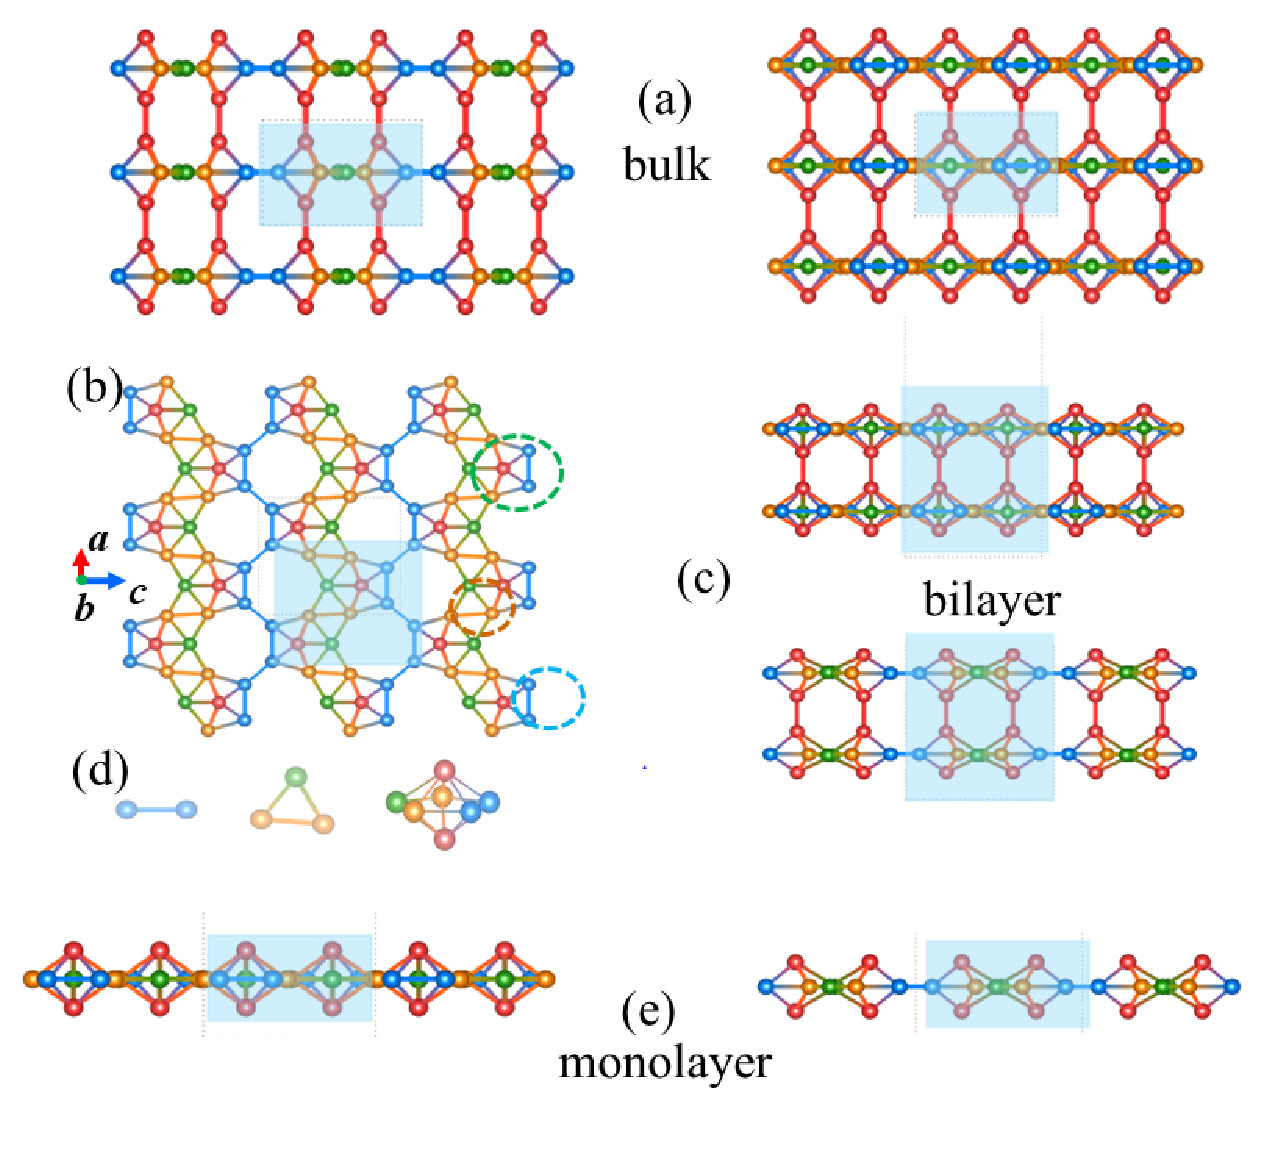
\includegraphics[width=0.8\linewidth]{Figure1-structures.eps}
	\caption{Atomic structure of o-B14: (a) side views and (b)
	top view of the bulk structure. 
	The unit cell is highlighted in pale blue.
The B atoms are grouped into three groups, G2, G3 and G7,
following Ref.~\cite{han2023superconducting} 
	which relate to the two (circled in blue), three (circled in orange) and
	seven (circled in green) B atoms. The atoms in these groups are 
	sketched in (d). The two side views of the bilayer (c) and
	monolayer (e) structure are also shown. The top view is the same as (b).}
    \label{fig-bulk}
\end{figure}

\begin{table}
\caption{Lattice constants, $a$, $b$ and $c$,  and internal coordinates
		of bulk o-B14~\cite{han2023superconducting}.  
		}
\centering
	\begin{tabular}{ccc}
\hline
	o-B14 & $a=5.6970$  (Å) & B1 (4x) (0.52123, 0.50000, 0.63796) \\
	      & $b=4.0479$  (Å) & B2 (4j) (0.60090, 0.50000, 0.89991)  \\
	      & $c=6.2042$  (Å) & B3 (4k) (0.75000, 0.79171, 0.72973) \\
& $\alpha = \beta =\gamma = 90^o$ & B4 (2f) (0.25000, 0.50000, 0.52367) \\
\hline
\end{tabular}
\label{tab-1}
\end{table}

\begin{figure}
\includegraphics[width=0.6\linewidth]{fig-bulk-bands-BZ.eps}
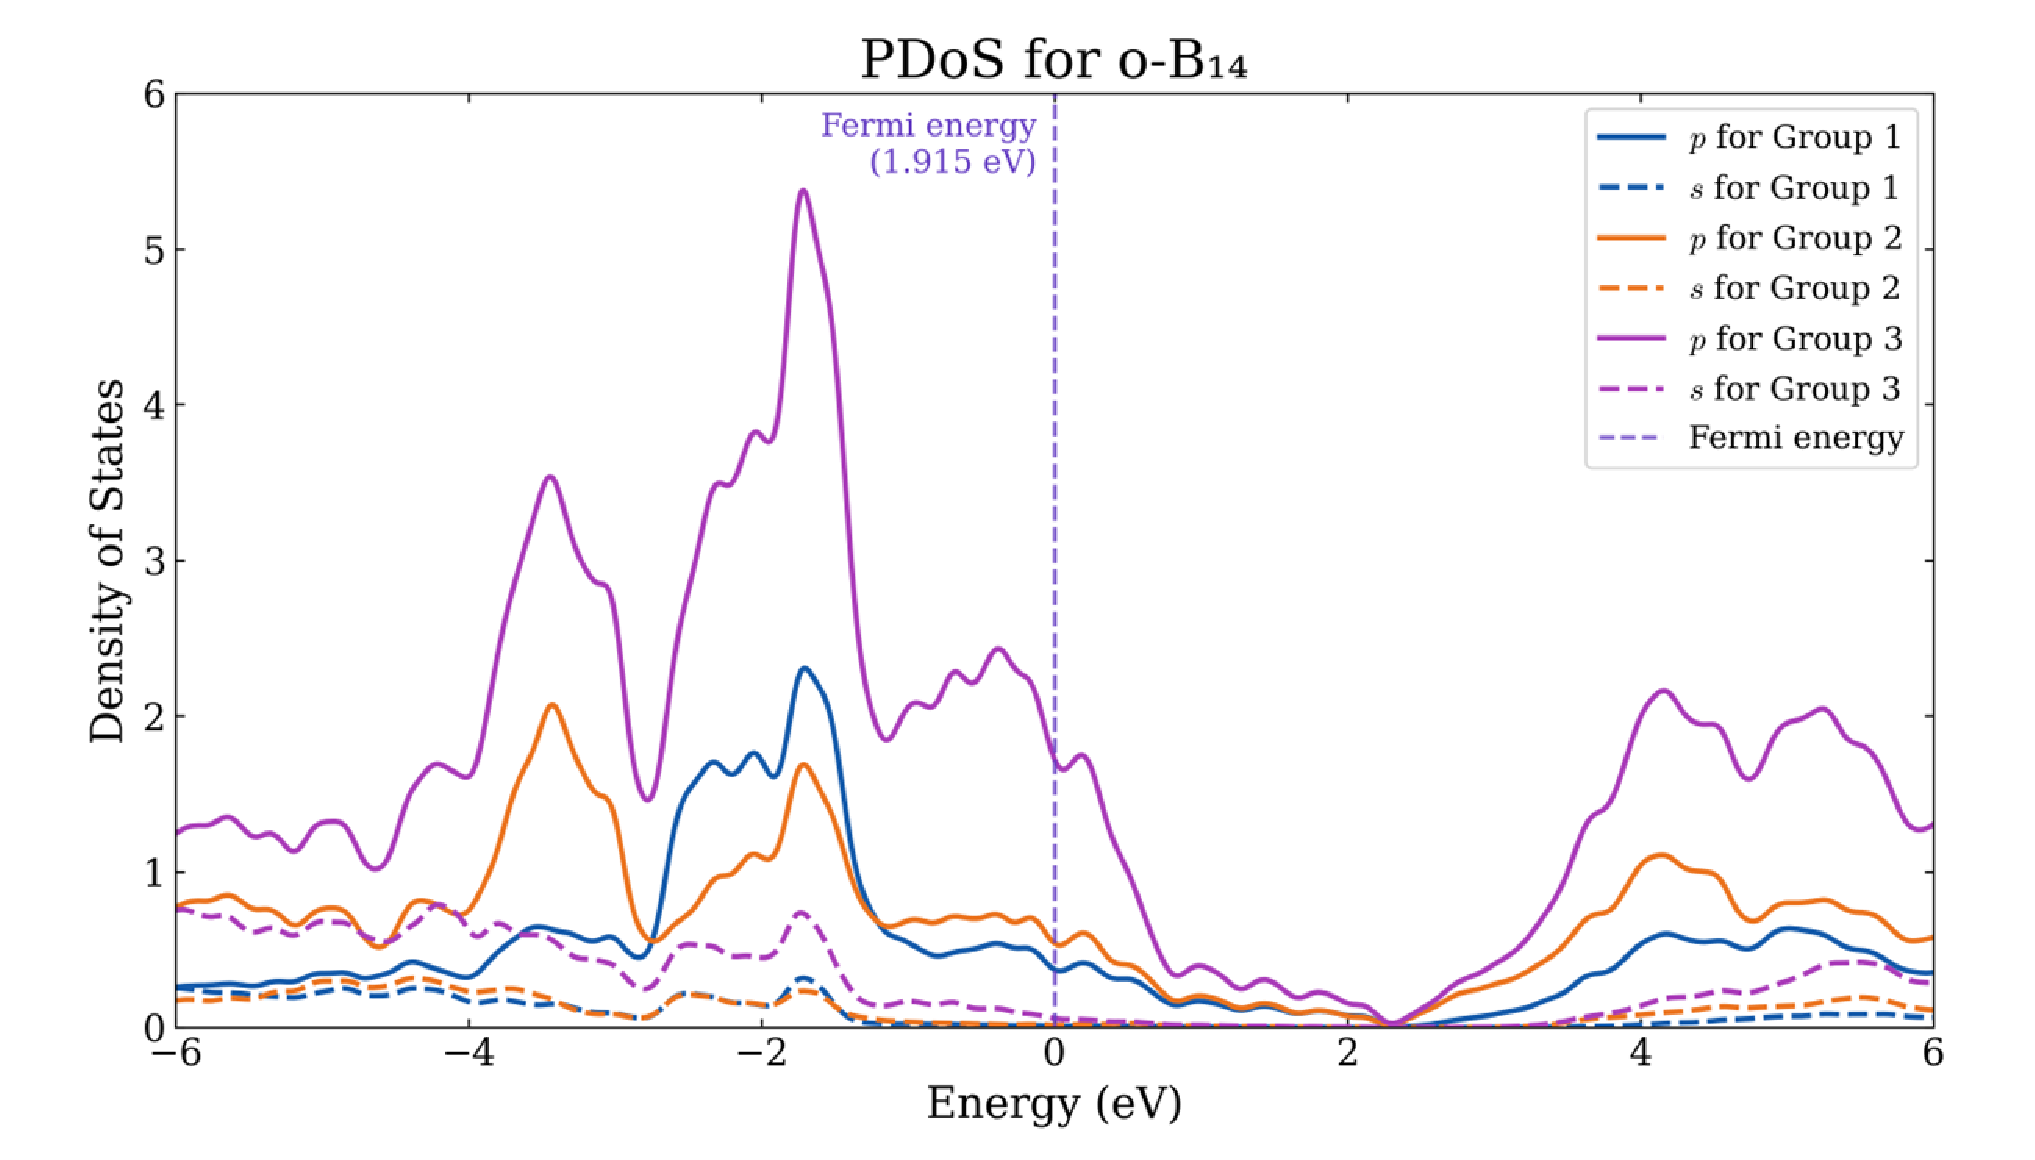
\includegraphics[width=0.6\linewidth]{fig-bulk-dos-groups.eps}
	\caption{Band structure of bulk o-B14  and the 
	Brillouin zone with
	high symmetry {\bf k}-points labelled (upper). State-projected density-of-states for bulk o-B14 with the different groups of 
B atoms indicated by colour, as defined in Fig.~\ref{fig-bulk}d (lower). }
    \label{fig-bs-bulk}
\end{figure}

\subsection{Monolayers and bilayers: Atomic and electronic structure, energetics}

\subsubsection{Structural Properties}
	The atomic structure of the bilayer and monolayer is shown in 
	Fig.~\ref{fig-bulk}c and 1e, respectively, where
	a vacuum region of $\sim$22~\AA\,
	in the direction perpendicular to the surface is included.	
	The H-terminated bilayer structure is 
	shown in Fig.~\ref{fig-H-term}a, where the H atoms are adsorbed 
	on top of the 
	B atoms of the bi-pyramids.
	We also considered the hollow-bridge site for hydrogen atom adsorption, located between the two apical B atoms on each side of the layer (cf. Fig.~S7). This adsorption site, however, was found to be metastable, and notably less favorable (by 1.57 eV, monolayer and 2.61 eV, bilayer per H atom) than the top site.

\begin{table}
\caption{Lattice vectors $a$ and $b$ of the various 2D systems, interlayer B-B distance, cohesive energies ($E_{c}$) adsorption energy
	of hydrogen atoms on the monolayer and bilayer 
	($E_{ad}$) and electronic nature. ``M'' stands for metallic,
	``FM" for ferromagnetic and ``SC'' for semiconducting.}
\centering
 \begin{tabular}{ccccccc}
\hline
	System &  $a$ & $b$ & Interlayer & $E_{c}$ &$E_{ad}$ & Nature \\
	&   &  &  B-B (\AA) &  & & \\
\hline
Monolayer       &5.700 & 6.314  &-&$-6.12$ &- &  AFM-SC\\
H-Monolayer       &5.694 & 6.134  &-& - &-1.450 &  M\\
Bilayer         &5.719 & 6.349  &1.693 &$-6.35$ &-& SC\\
H-Bilayer       &5.680 & 6.147  &1.645 &- & $-1.525$ & M\\
Bulk            &5.697 & 6.204  &1.686 &$-6.16$ & & M\\
	 $\alpha '$-monolayer~\cite{niu2024electronic}            & & & &$-6.00$ & & M\\
\hline
\end{tabular}
\label{tab-layers}
\end{table}


	The optimised structural parameters of the systems
	are given in Table~\ref{tab-layers}, 
	along with the cohesive and adsorption energies, and the
	electronic nature. 
	Compared to bulk o-B14, it can be seen that the in-plane lattice 
	constants of the monolayer and bilayer are slightly larger, as is
	the 
	bond length of the interlayer B-B distances 
	of the bilayer
	(by 0.4\%). On the other hand, the in-plane lattice constants for 
	the H-terminated monolayer and bilayer are 
	slightly smaller compared
	to the bulk, as is the interlayer B-B distance (by 2.4\%). 
	The cohesive energy of the monolayer and bilayer  are  $-6.12$ eV and
	$-6.35$ eV, respectively. These values can be 
	compared to bulk o-B14 of $-$6.16~eV and to that of 
	the $\alpha '$ phase of borophene ($-$6.39 eV) 
	which we reported in our earlier
	publication~\cite{niu2024electronic}, calculated with the same approach.
	The adsorption energy of the hydrogen atom on the bilayer is 
	$-1.525$ eV, slightly stronger than on the monolayer which is $-$1.450 eV.

\begin{figure}
    \centering
    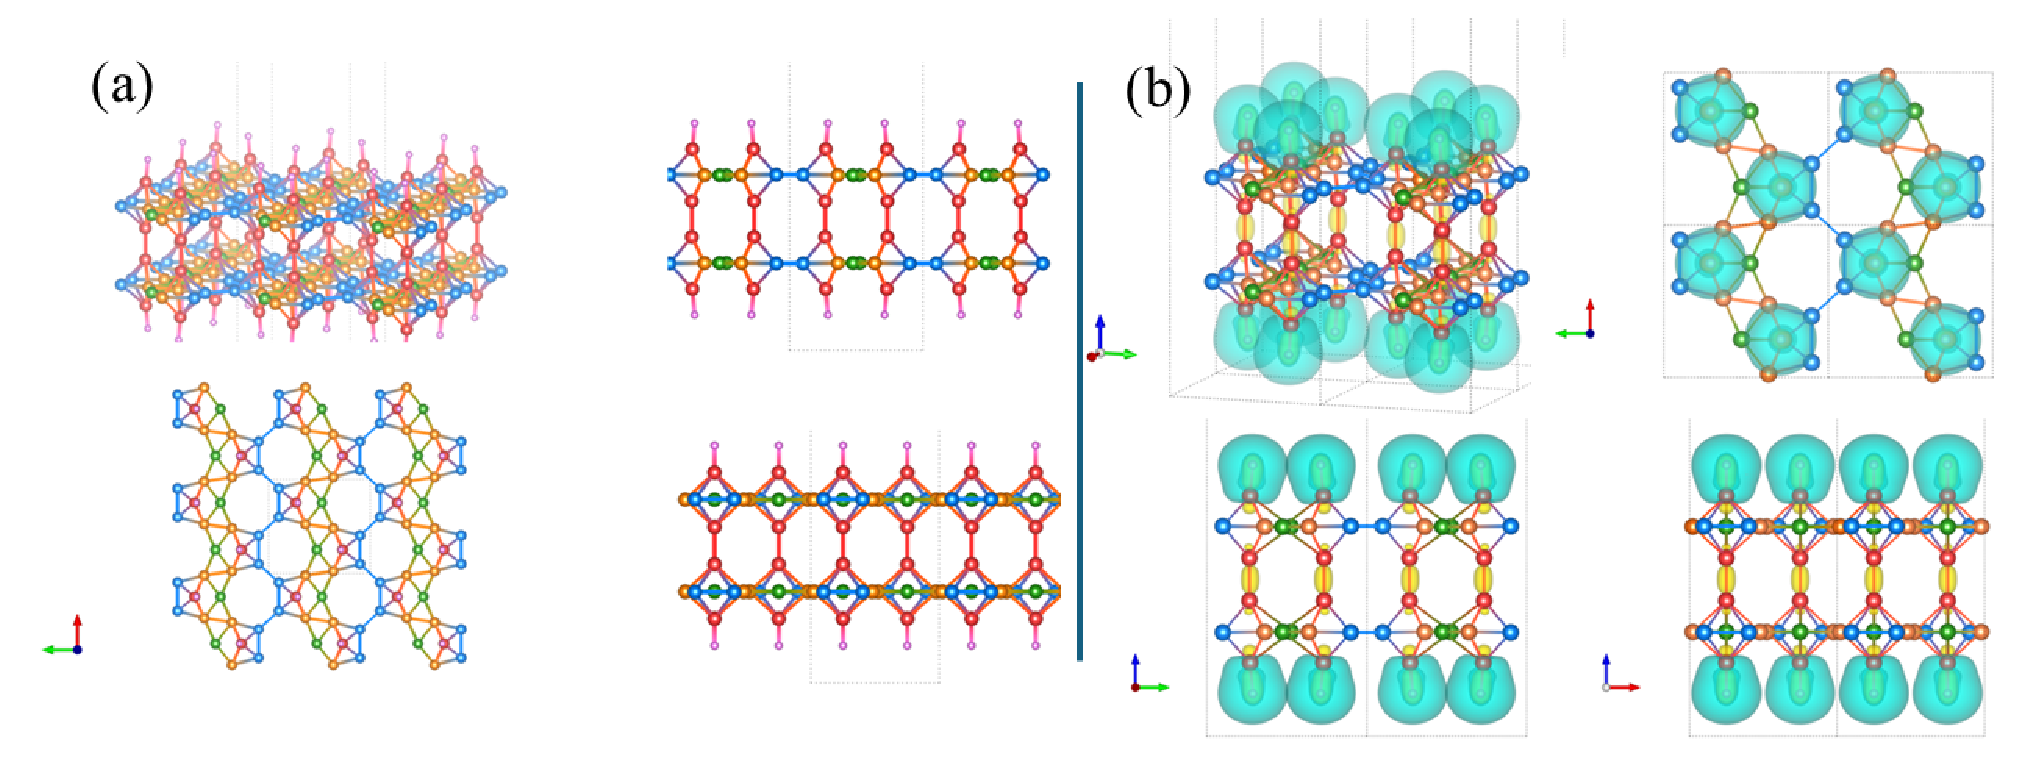
\includegraphics[width=1.0\linewidth]{fig-new-H-term-all.eps}
	\caption{Atomic structure of the hydrogen-terminated bilayer 
	structure (a) showing a top view of the $(3\times 3)$ supercell. 
	(b) The charge density difference ($\Delta \rho(\bf{r}))$ showing a $(2\times 2)$ supercell, calculated 
	using Eq.~\ref{eqn:charge_difference} on adsorption of 
	hydrogen.
	Regions of charge accumulation are
	shown in yellow and regions of charge depletion are shown in blue. 
	The isosurface level is $1.5\times10^{-4} e$ a$_{0}^{-3}$.}
    \label{fig-H-term}
\end{figure}

\subsubsection{Dynamic stability: Phonon dispersion}

	To investigate whether the monolayer and bilayer structures, both with and without hydrogen adsorption are dynamically stable, 
	the phonon dispersion curves are calculated. The results,
	obtained from finite differences using $(3\times3)$ supercells,  are shown in Fig.~\ref{fig-phonon} 
	for the monolayer and bilayer. It can be seen that no imaginary frequencies are present and thus they are predicted to be dynamically stable. For the hydrogen terminated systems, we find that
	the H-bilayer is dynamically stable, while the H-monolayer is not. This can be seen from presence of imaginary frequencies for the latter, but not the
	former, in Figs.~S8 and S9 of the SI.
	Based on these results, the hydrogen-terminated monolayer is not 
	considered further.
	Using {\em ab initio} molecular dynamics (AIMD) calculations
	for a temperature of 400~K (using VASP), we also verified that the H-bilayer was thermodynamically stable as can be seen from Fig.~S10.
	
\begin{figure}
    \centering
    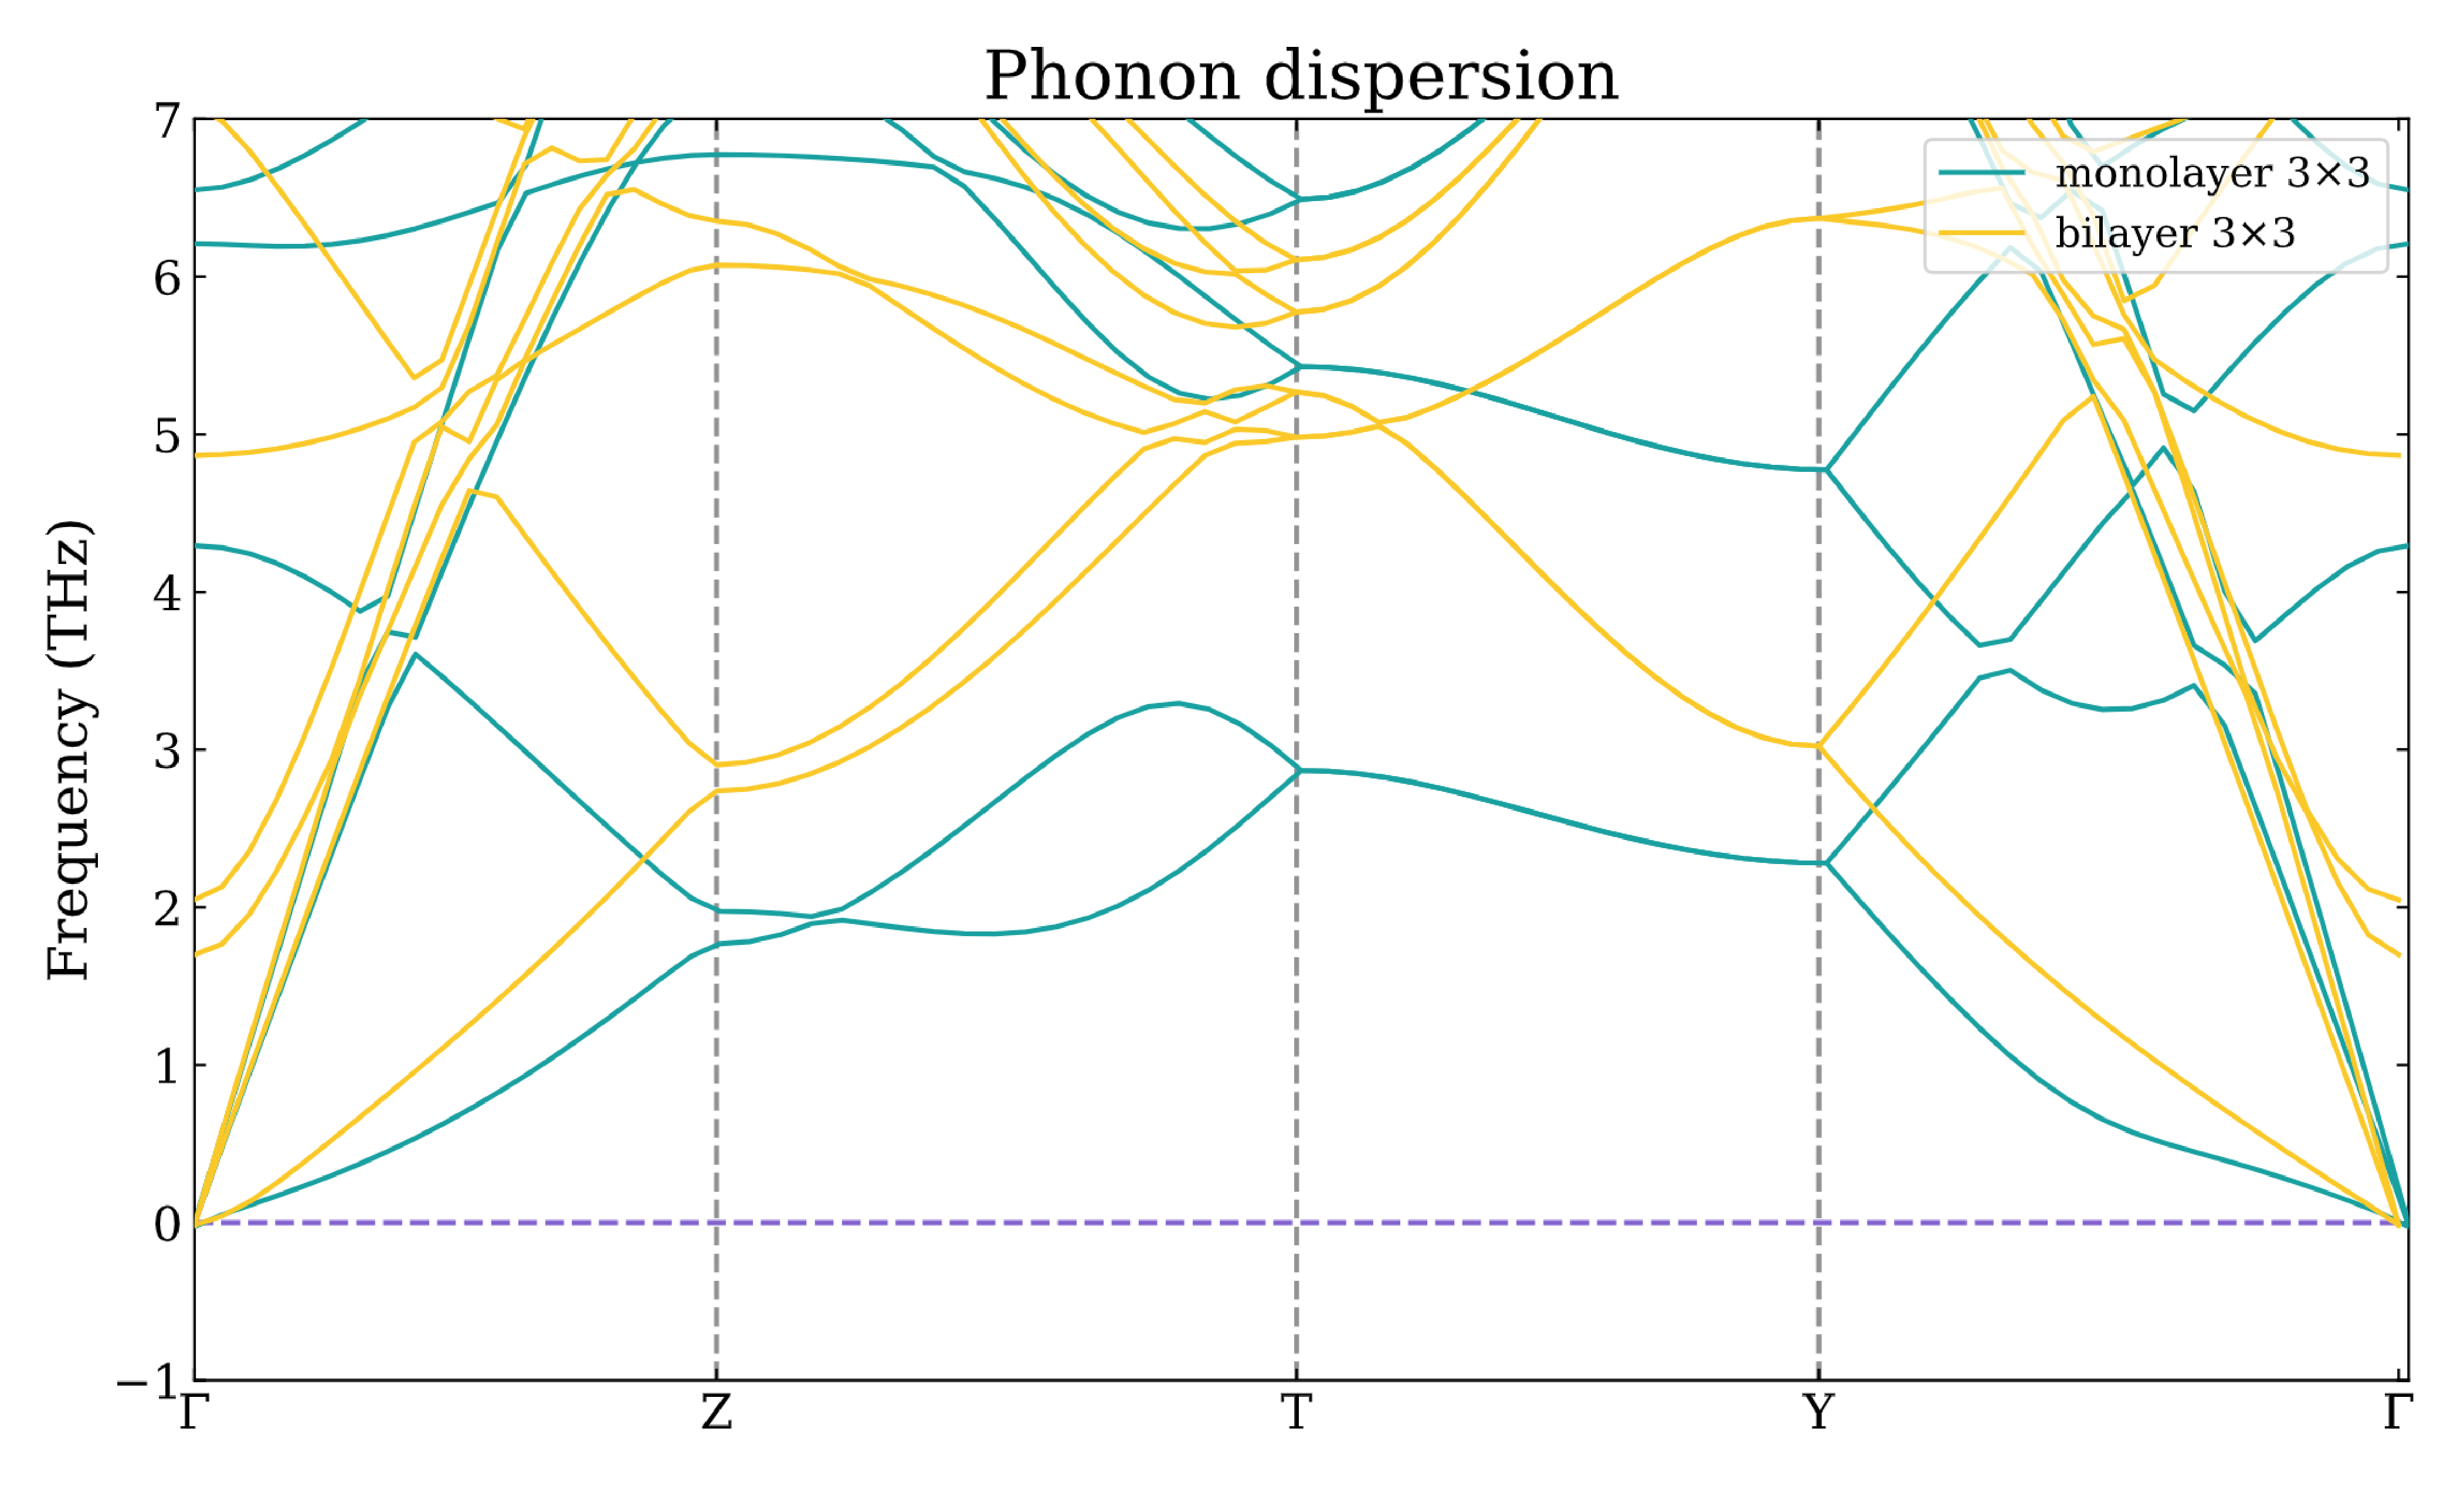
\includegraphics[width=0.7\linewidth]{fig-phonon-bilayer-monolayer-3x3.eps}
	\caption{Phonon dispersion curves for monolayer and bilayer o-B14,
	as calculated from finite differences using a $(3\times3)$ supercell.}
    \label{fig-phonon}
\end{figure}


\subsubsection{Electronic properties}

The charge density difference distribution for the adsorption of hydrogen
	on the surface of the bilayer is shown in 
	Fig.~\ref{fig-H-term}b. It can be seen that there is a significant depletion 
	of electron density around the H atoms and an increase both in the interlayer B-B 
	bonds, as well as in the $p_{z}$ orbital of the uppermost bipyramid B 
	atom directed to forming a bond with the H atom 
	(partially hidden within the large depletion area).
	The increase in electron density between the interlayer B-B bond, is consistent
	with the slightly smaller distance compared to without H adsorption.


The band structure of the monolayer 
	is shown in Fig.~\ref{fig-bs-monolayer}  as calculated using
	the HSE06 functional with spin-polarization. It is found that the antiferromagnetic (AFM) configuration (Fig.~5, upper) is more favourable 
	that the ferromagnetic (FM) configuration (Fig.~5, center and 
	Fig.~S11 (PBE)) by 0.02 eV. 
	A small band-gap of 0.105 eV opens up in the AFM case. 
\begin{figure}
    \centering
    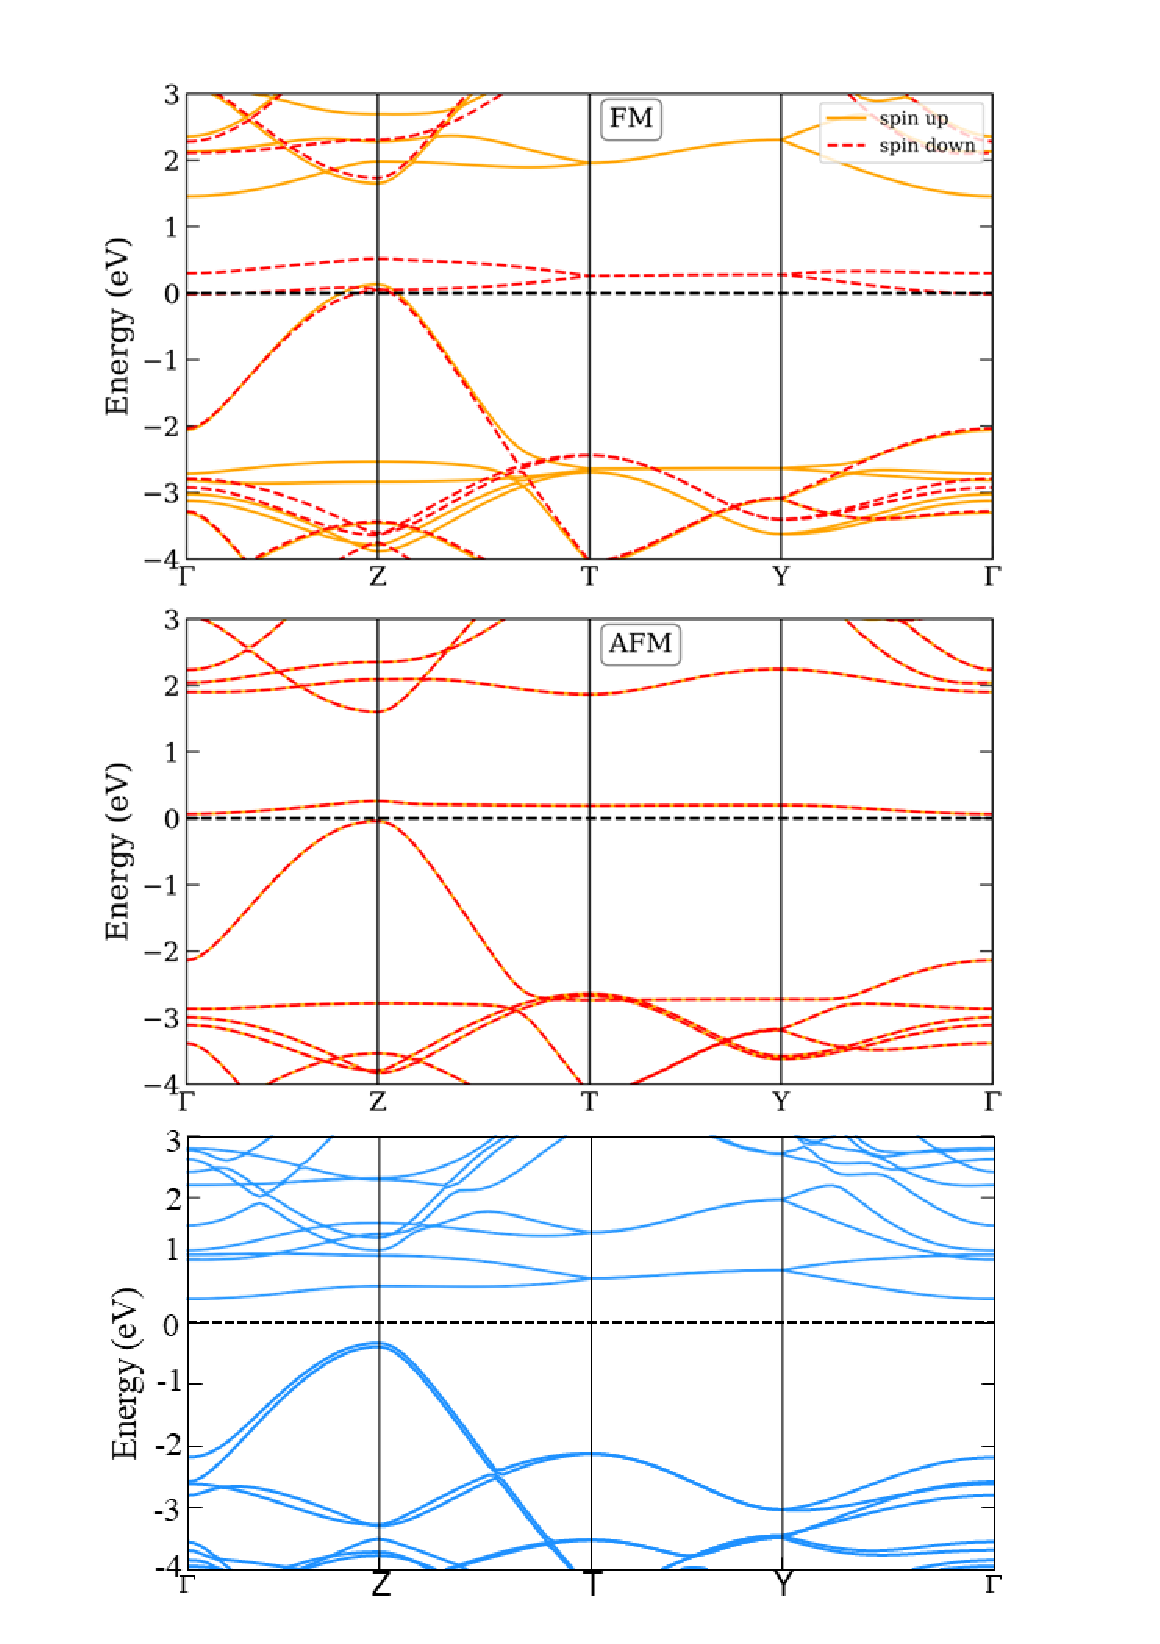
\includegraphics[width=0.6\linewidth]{fig-mono-bilayer-bands.eps}
	\caption{Spin-polarized band structure of the monolayer as calculated using the HSE06 functional: FM, upper and AFM center. 
	Band structure of the bilayer calculated using 
	the HSE06 functional (lower). 
	The Fermi energy is the energy zero and for the semiconducting systems,
	the energy zero is
	in the middle of the band-gap.}
    \label{fig-bs-monolayer}
\end{figure}
In the non-magnetic state, the
system is metallic and exhibits a high DOS at the Fermi level 
which is related to flat bands 
throughout the Brillouin zone, and particularly along the T-Y direction 
(Figs.~S12, S13).
Since a large DOS at the Fermi level often suggests that a material is 
prone to undergo transitions to more stable ground states, such as forming 
superconductors, ferromagnets, or experiencing structural distortions like 
the Jahn-Teller effect (cf. Fig.~S14), we tested all these aspects.
As mentioned above, 
it is found that the structure is magnetic, with a magnetic moment of
0.262 $\mu_B$ on each apical B atom. 
For the FM case, fixed-spin calculations (cf. Fig.~S15) shows a total
magnetic moment of the unit cell of around 2~$\mu_B$.
The DOS  of the FM structure clearly shows the significant spin-splitting (spin-up and spin-down) of the states related to the apical B atoms 
(Fig.~S16, upper).
The DOS for the AFM ordering is shown in Fig.~S16 (lower). 

For the AFM case,
the spatial distribution of the wavefunction of the highest
occupied, and 
lowest unoccupied states at a {\bf k}-point mid-way 
along the high-symmetry line 
T-Y in the BZ is shown in Fig.~6a, along with the total spin 
density, Fig. 6b. It is apparent that the apical B atoms of the bipyramid are responsible
for the magnetic behavior of the system where they have a magnitude 
0.262 $\mu_B$. 
The analogous result for the FM ordering is shown in Fig.~S17.
The energetic preference for AFM ordering over FM ordering can be understood in terms of the competition between electron hopping and exchange interactions. In the AFM configuration, virtual hopping between neighboring magnetic sites is enhanced because electrons can delocalize onto oppositely aligned spins without violating the Pauli exclusion principle, leading to a greater kinetic-energy lowering. In contrast, FM alignment restricts such virtual hopping processes and reduces the associated kinetic-energy gain, rendering the AFM state energetically more favorable.

The band structure and DOS of the bilayer is shown in Fig.~5 (lower), as 
calculated using the HSE06 functional. The bilayer is an indirect semiconductor with a band-gap
of 0.67~eV, where 
the valence band maximum (VBM) is at the Z-point and the conduction band 
minimum at the $\Gamma$-point. 
Using the PBE results in a semi-metal. 
On terminating the bilayer structure with hydrogen, the band structure changes
dramatically. Specifically, it can be seen from Fig.~\ref{fig-bs-bilayer-H} 
that the system is now metallic and bears some resemblance to that of the 
bulk band structure. 


\begin{figure}
    \centering
    \includegraphics[width=0.8\linewidth]{Figure_Monolayer_AFM.eps}
	\caption{(a) The highest 
	occupied and lowest unoccupied spin-up and spin-down states 
	of the monolayer in the AFM state at 
	a {\bf k}-point midway along the high symmetry T-Y direction (isosurface is 1$\times$10$^{-7}$ e/\AA$^{3}$).
	(b) The spin-density of the monolayer. The isosurface is 0.005 e/\AA$^{3}$.}
    \label{fig-spin-state}
\end{figure}


\begin{figure}
    \centering
    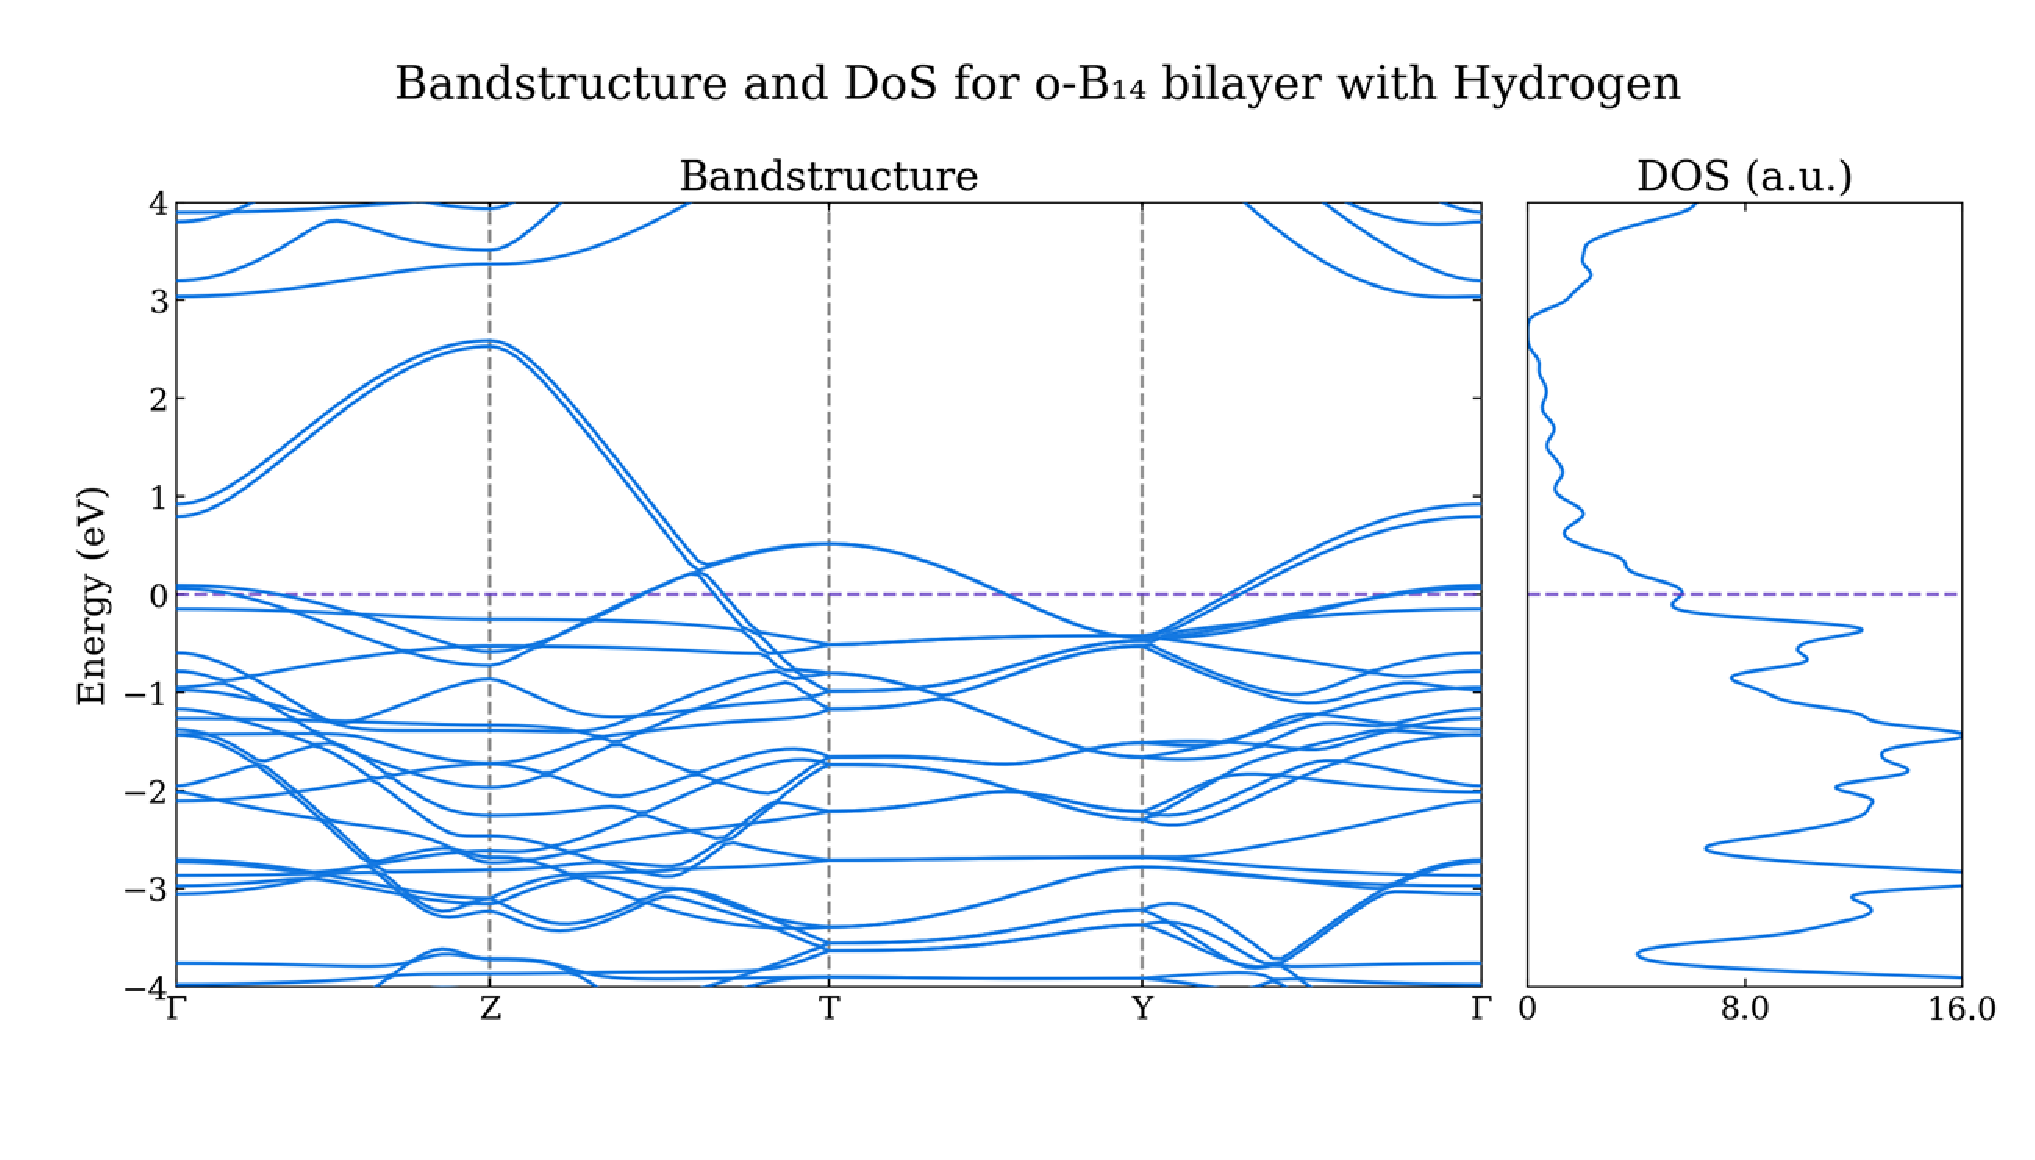
\includegraphics[width=0.8\linewidth]{fig-bilayer-h-dos.eps}
	\caption{Band structure and total density-of-states for the bilayer with
	hydrogen termination.}
    \label{fig-bs-bilayer-H}
\end{figure}
\subsection{Superconducting properties of o-B14}
The (conventional) superconducting properties of 
bulk o-B14, the monolayer and H-terminated bilayer are investigated.
The bilayer is not considered due to its semiconducting nature.
We first confirm that the atomic relaxation obtained using Quantum ESPRESSO (QE) yields very similar results to those obtained by VASP, namely, we obtain: lattice constants (a, b): QE 5.66, 6.12 \AA; VASP 5.68, 6.14 \AA; interlayer distance: QE 4.13 \AA;  VASP 4.11 \AA, and H-B distance: 1.19 \AA,  in both cases.
For the bulk phase, an electron phonon coupling strength
of $\lambda$ = 0.931 is obtained, corresponding to an estimted Allan-Dynes superconducting temperature of $T_c$ = 28.2 K, 
consistent with the prior report of 29.1~K~\cite{han2023superconducting}. 
The hydrogen-terminated 
bilayer exhibits a slightly higher coupling strength ($\lambda = 1.01$) but 
a lower $T_c$ = 18.5 K, which may be attributed to the phonon softening 
effects arising at higher electron phonon coupling strengths~\cite{migdal1958interaction,marsiglio2020eliashberg,eliashberg1960interactions}. 
The monolayer phase yields $\lambda$ = 0.05 and a negligible $T_c$, 
indicating the absence of significant phonon-mediated superconductivity. 

From the anisotropic Migdal-Eliashberg equations,
analysis of the superconducting gap evolution further supports these 
findings: the bulk gap is observed to close around $T_c$=31.3 K
(Fig.~8a), and the bilayer gap around $T_c$ = 24.3 K (Fig.~8b). 
Overall, these results suggest that o-B14 is unlikely to possess 
conventional superconductivity in the monolayer phase owing to the 
extremely weak electron phonon interactions, whereas the bulk and 
hydrogen-terminated bilayer possess credible phonon-mediated 
superconducting states corresponding to transition temperatures 
ranging between 20 - 30 K.
\begin{figure}
    \centering
	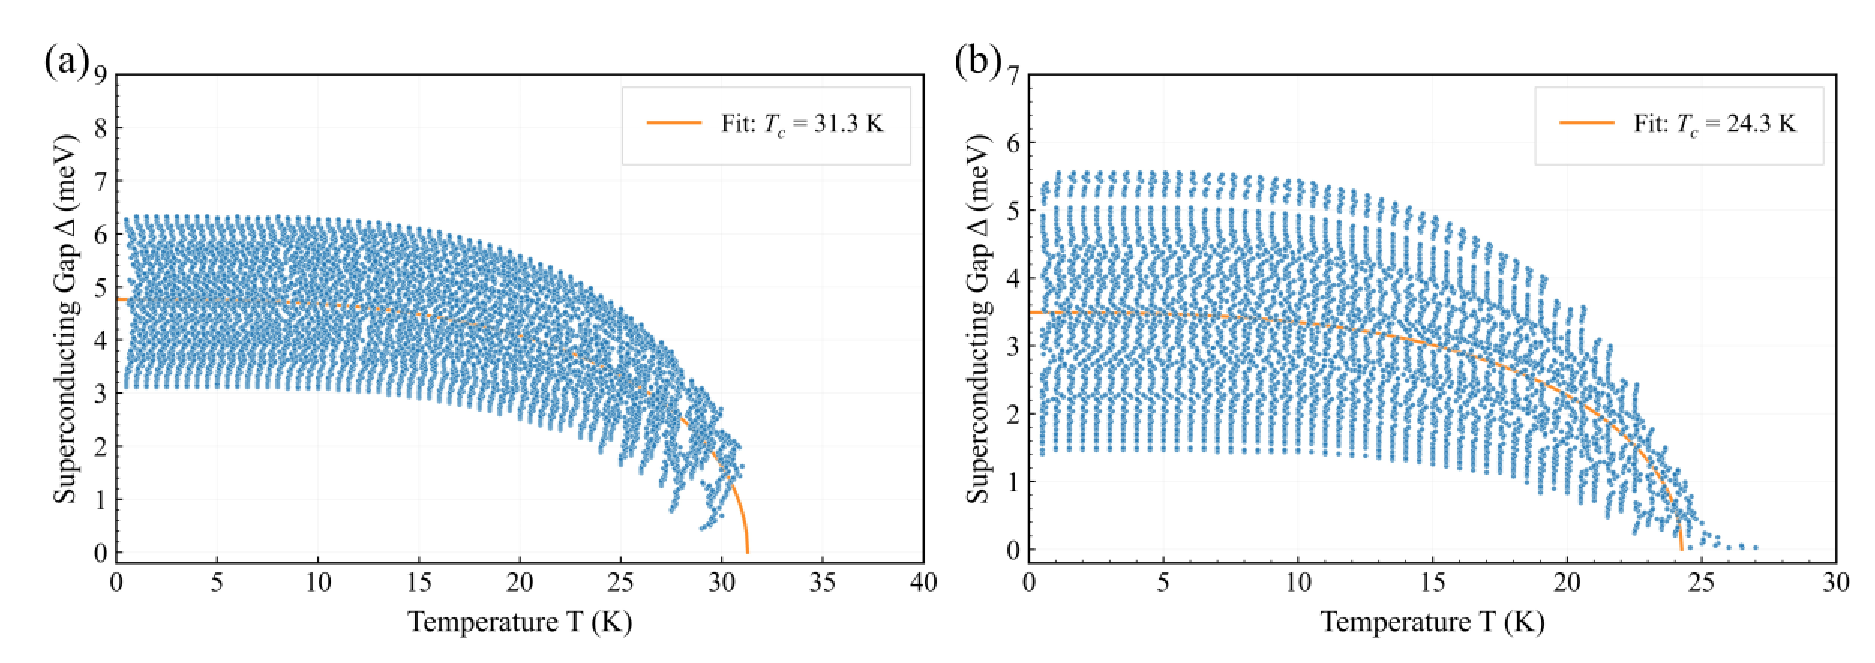
\includegraphics[width=0.7\linewidth]{fig-supercond-Figure-10.eps}
	\caption{Superconducting gap versus temperature for (a) bulk o-B14 and
	(b) hydrogen-terminated bilayer o-B14.}
    \label{supercon}
\end{figure}
\subsection{Optical properties}
\begin{figure}
    \centering
	\includegraphics[width=1.0\linewidth]{fig-new-dielec-func.eps} 	
\caption{Real and imaginary parts of the dielectric function
	for the bulk and 2D o-B14 structures for the $xx$, $yy$ and $zz$ directions.}
    \label{fig-dielec}
\end{figure}
The optical properties are now considered. In particular, the 
real ($\epsilon_1$) and imaginary part ($\epsilon_2$) of the dielectric 
function are calculated, and from them  the other optical properties are 
determined (cf. Eqs.~(1-5) of the SI). 
The imaginary part,
$\epsilon_2$, is a measure of light absorption as a consequence of 
neutral and plasmonic charge excitations and 
$\epsilon_1$ is a measure of the 
strength of the dynamical screening effects arising from charge excitations. 
Metallic character is indicated by a  negative value of $\epsilon_1(\omega)$
for the corresponding 
ranges of the electromagnetic spectrum.
For a plasmon resonance, $\epsilon_1(\omega)$
must typically cross from a negative value to positive with increasing energy.
This behavior indicates a restoring force becoming insufficient to fully 
screen the external field, a condition where plasma oscillations (plasmons) 
can be excited.  In metals, at low frequencies,
$\epsilon_1 (\omega)$ is usually negative, indicating a metallic 
(screening) response.
As it increases, the ability to screen weakens, and
  $\epsilon_1 (\omega)$ increases.
A plasmon resonance is reached when
$\epsilon_1 (\omega)=0$ 
and when $\epsilon_2 (\omega)$ is close to zero, indicating the onset of collective charge oscillations.
The plasmon will then be optically active, i.e., it 
strongly couples to light or other external probes and appears as a 
distinct peak in spectra (e.g., reflectivity, electron energy loss
spectroscopy (EELS), absorption).


Figure~\ref{fig-dielec} shows 
the real and imaginary parts of the dielectric function for all the structures 
considered for the $xx$, $yy$ (in-plane) and $zz$ (out-of-plane) components.
It can be seen that
each component of the dielectric function is different, indicating 
that the response of the structures to light is highly dependent on the
polarisation direction of incoming light.
That is, the systems exhibit anisotropy, leading to polarization-dependent 
optical properties and directionally selective light–matter interactions.

For photon energies less than around 2.0~eV, the $xx$- and $yy$-components differ for the bulk and hydrogen-terminated bilayer
in that $\epsilon_1$ for the $xx$-component
is negative in part of this region while the $yy$ is not.
It also can be seen that for some range of energies the monolayer, hydrogen
terminated bilayer, and bulk 
system behave as indefinite media, for which in-plane and out-of-plane $\epsilon_1$
are of opposite sign, namely in the region below 2.0~eV for the former
two systems, and 
between 6.0~eV and 10.0 eV for the latter, signalling directional plasmonic modes. 

The real part of the dielectric function for the $xx$-component,
shows that there is a plasmon for the bulk, monolayer and the
hydrogen terminated bilayer, in the region between 0.5-1.5~eV, where the imaginary part is correspondingly
very low. For the monolayer, this plasmon persists in the $yy$-direction and
is even more pronounced, while for the bulk and hydrogen-terminated bilayer,
it is not present.
Interestingly, in the out-of-plane $zz$-direction, the presence of plasmons
as
indicated by the negative values of $\epsilon_1(\omega)$, is seen 
for the H-terminated bilayer, monolayer and the  bilayer 
at around 1.5~eV, 3.6~eV and 6.0~eV, and 5.0~eV, respectively, which 
correspond to the significant peaks in the energy loss spectrum in Fig.~10 (lower).

Peaks in the imaginary part of the dielectric function signal strong absorption due to electronic transitions, typically interband excitations. 
The energy, width, and intensity reflect the band structure and 
optical activity.
In the present case, except for the bilayer, characteristic metallic
behaviour is observed, namely, a large value
at low energies, due to the intraband (Drude) absorption from free electrons. 
The bilayer, on the other hand, is small until interband transitions begin,
consistent with its semiconducting nature.
\begin{figure}
    \centering
    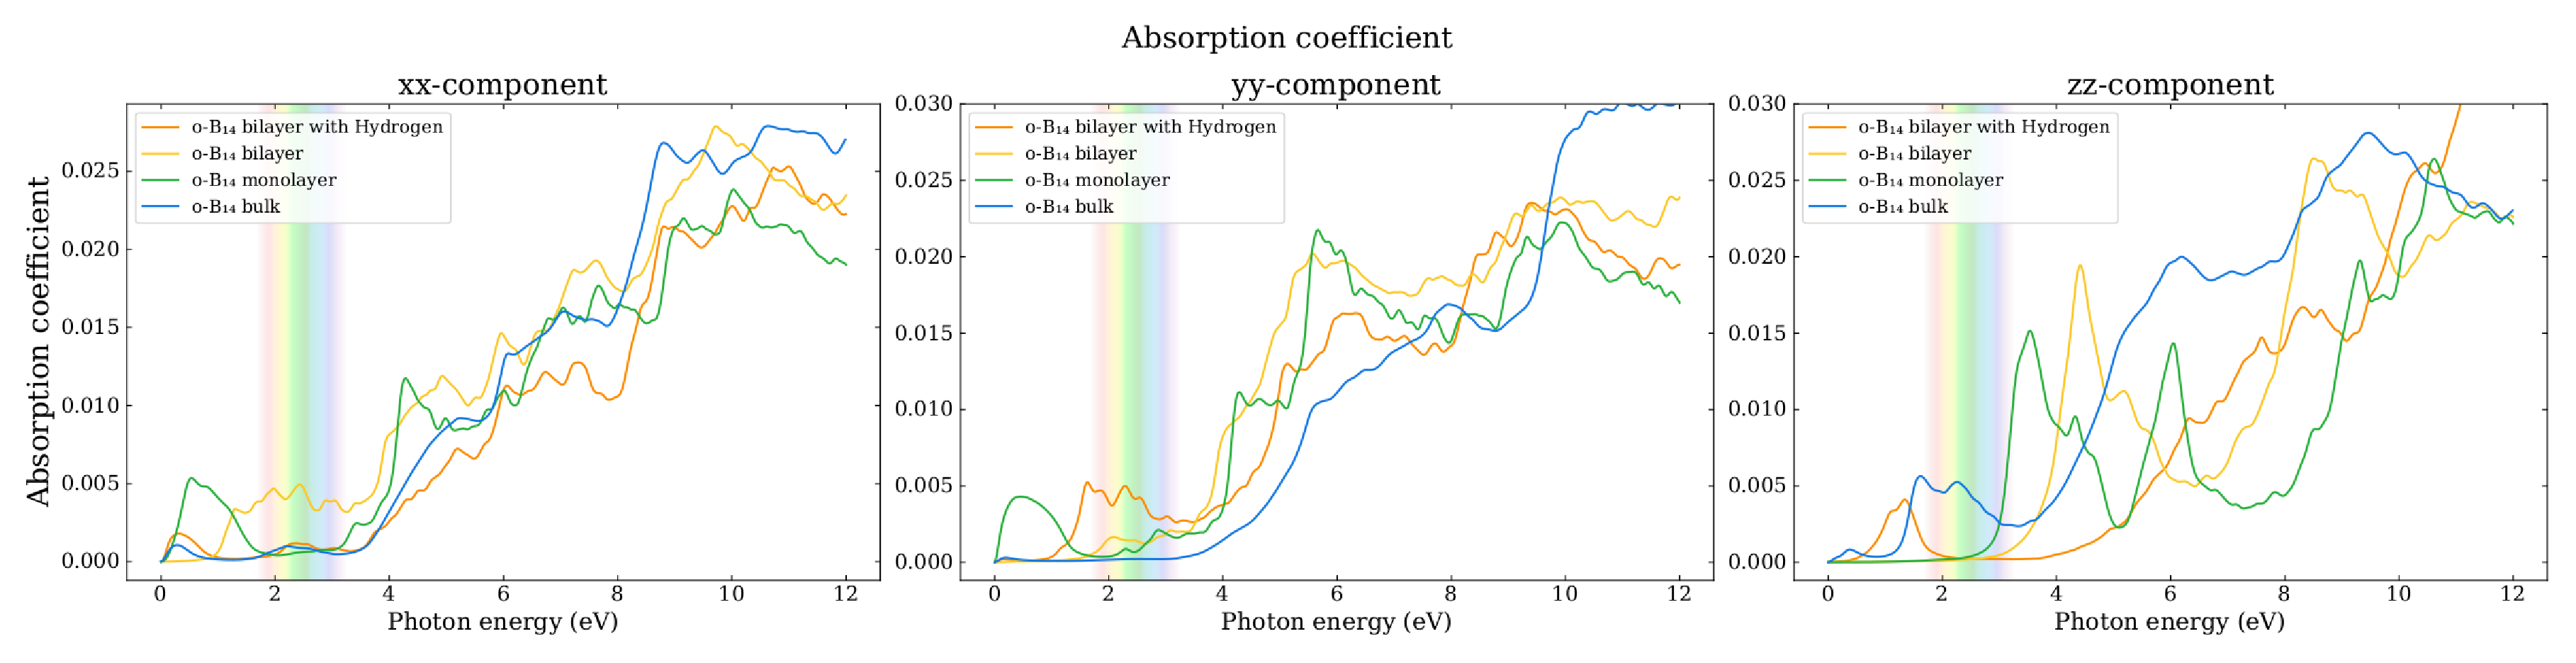
\includegraphics[width=1.0\linewidth]{fig-new-6.1_absorption.eps}
    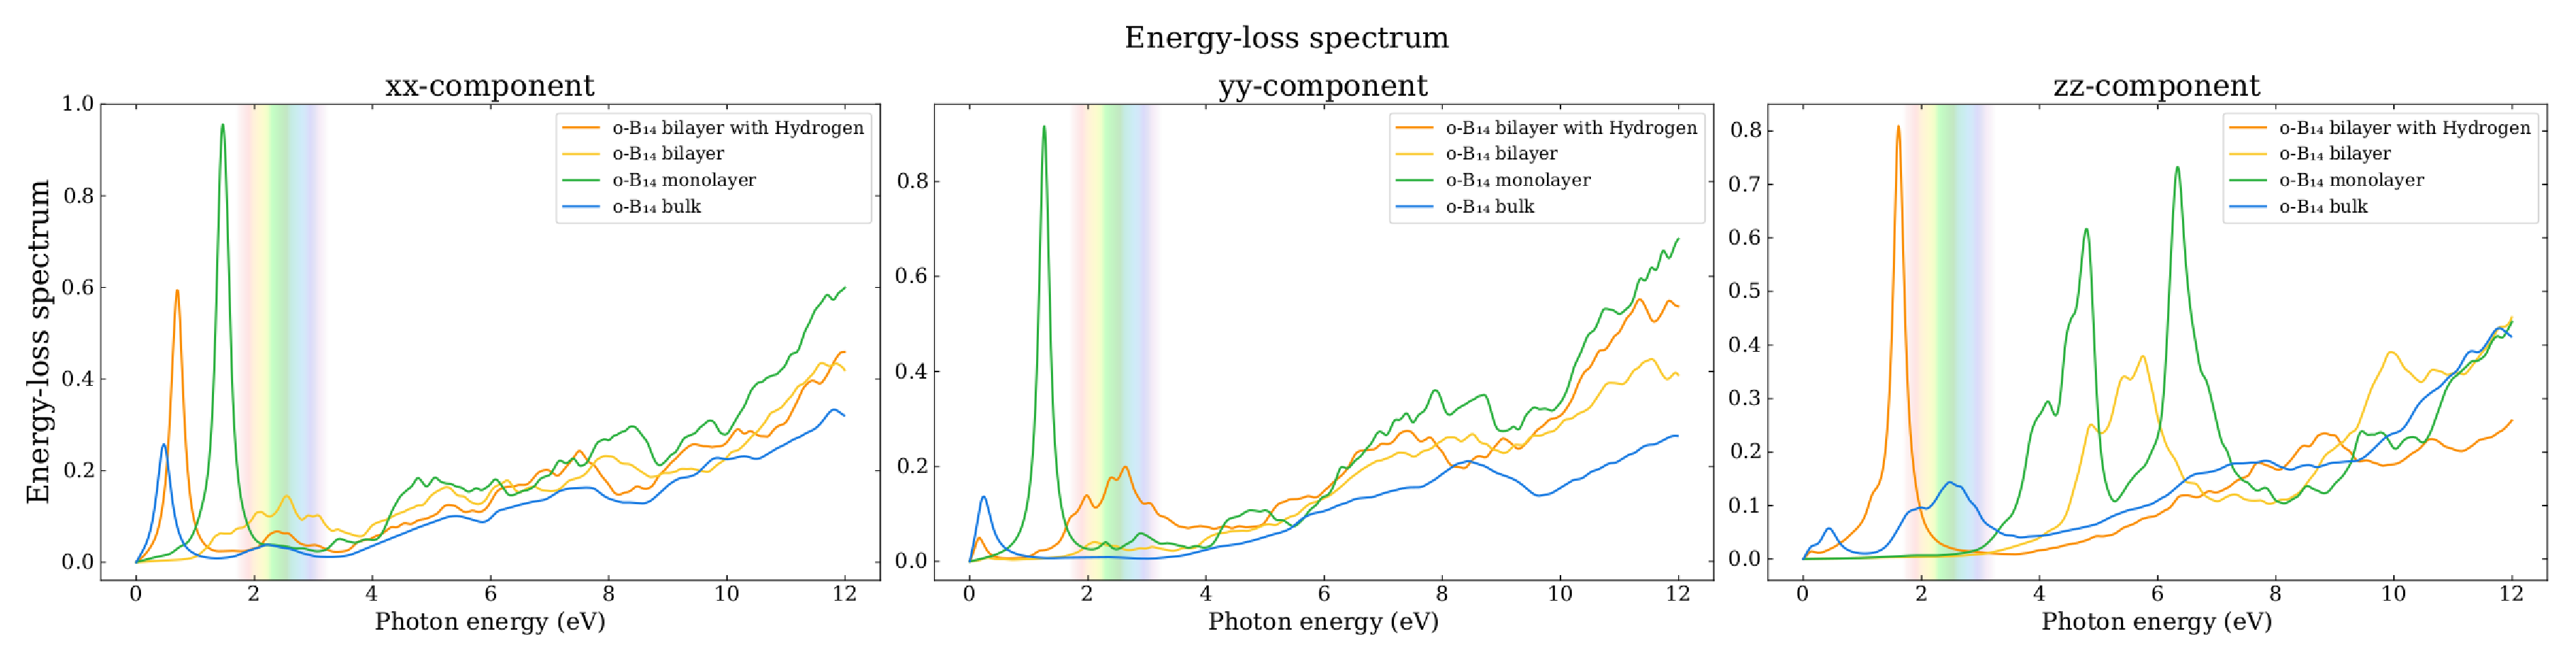
\includegraphics[width=1.0\linewidth]{fig-new-6.5_energy-loss.eps}
	\caption{The absorption (\AA$^{-1}$)and energy loss for the bulk and 2D o-B14 structures 
	for the in-plane ($xx,yy$) and out-of-plane ($zz$) directions.}
    \label{fig-absorp-enloss}
\end{figure}
The dielectric tensor characterizes how the polarization of the 
material changes in response to an applied electric field. For an incident 
photon, the tensor components represent the response of the 
material to the electric field component of the photon
along different directions, 
e.g. the element $\epsilon_{yx}$ and $\epsilon_{xy}$ describe the  response 
to an electric field applied along the $y$-direction, resulting in polarization along the $x$-direction and vice versa. 
A non-symmetric dielectric tensor 
i.e $\epsilon_{yx}\neq \epsilon_{xy}$ 
implies time-reversal symmetry is broken and can lead to 
Faraday rotation (the rotation of light polarization 
during propagation)
circular dichroism, and non-reciprocal light propagation. This results in
light behaving differently depending on the direction it travels through 
a material. 
For all systems studied here, however, the off-diagonal components of the dielectric 
tensor are zero. 

In order to further explore the optical properties of the o-B14 based 
structures, the absorption coefficient, loss function, reflectivity, refractive index, and extinction coefficient are calculated.
Figure~\ref{fig-absorp-enloss}  shows the absorbance and loss function for 
the various structures.
The absorption coefficient is directly proportional to 
the imaginary part of the dielectric function, where
the absorbance threshold corresponds to where 
$\epsilon_{2}(\omega)$ shows its first peak. 
For all but bilayer o-B14, the threshold is close to zero, corresponding to the 
metallic nature. With regard to the absorption coefficient,
in the visible region of the spectrum (1.7-3.3 eV) it can be seen that for the 
$xx$-, $yy$- and $zz$-components, the bilayer, H-bilayer, and bulk systems
have significantly the greatest value of absorption coefficient, respectively. 
The monolayer, on the other hand, exhibits strong absorption in the near-infrared and ultraviolet.
This value of around 0.005 \AA,(or 5$\times 10^{-5}$ cm$^{-1}$) 
is similar to that calculated for bulk silicon~\cite{saunders2024}, 
and notably larger than that reported for bilayer silicon as calculated by 
the same approach~\cite{saunders2024}.

The loss function in Fig.~\ref{fig-absorp-enloss} (lower)  exhibits several sharp 
peaks. 
For the $xx$-component, plasmon excitations can be
seen below 2.0~eV for the bulk, H-bilayer and monolayer, while for the 
$yy$-component, only the monolayer shows a strong excitation in this 
energy range. In the out-of-plane direction, there is a strong
peak for the H-bilayer below 2~eV, while the monolayer exhibits two strong features
at around 4.0~eV and 6.0~eV corresponding to the above-mentioned plasmons.
The bilayer also has a strong feature at about 5.0~eV. 

In Fig.~\ref{fig-reflec-refrac}, the reflectivity and refractive index are 
shown.
The reflectivity features directly reflect the electronic structure, where
the drops in it correlate with the edges of the above-discussed
plasmons.  
It can be seen that the trends in refractive index are similar to $\epsilon_1$, which indicates that the  effect of the real part of the dielectric function on the refractive index plays the leading role. 
The refractive index determines how much the path of light is bent, or refracted, when entering a 
material. Most transparent materials have refractive indices between 
one and two 
for visible light. 
The absolute refractive index of an optical medium is defined as 
the ratio of the speed of light in vacuum and the phase velocity (speed at which the crests of the wave move) of light in a material.  
It is possible for the phase velocity to travel faster than the speed of light in vacuum so the refractive index can be less than one.  
Near the plasmon resonance in 2D materials, the refractive index can drop below one due to the strong interaction between light and the plasmonic oscillations.
Metals can have a high refractive index at low photon energies 
due to strong absorption, and as the energy increases, 
the refractive index drops to values between one and two, 
particularly near, or beyond, interband transitions and the plasma edge. This change reflects how the material transitions from strongly reflective/absorptive (not transmitting light)
to partially transparent or weakly reflective at higher energies.

It can be seen  from Fig.~\ref{fig-reflec-refrac} 
(lower) that the refractive index for in-plane polarization is close to, and less than one for energies in the range of $\sim$0.5 - 1.5 eV for
the monolayer. For out-of-plane, this occurs at energies around 1.5~eV (H-bilayer), 3.6 and 6 eV (monolayer) and around 4.8 eV (bilayer).
This means that in these ranges of the electromagnetic spectrum, the structures are highly transparent, and it is in the region of where the plasmons occur. 
\begin{figure}
    \centering
    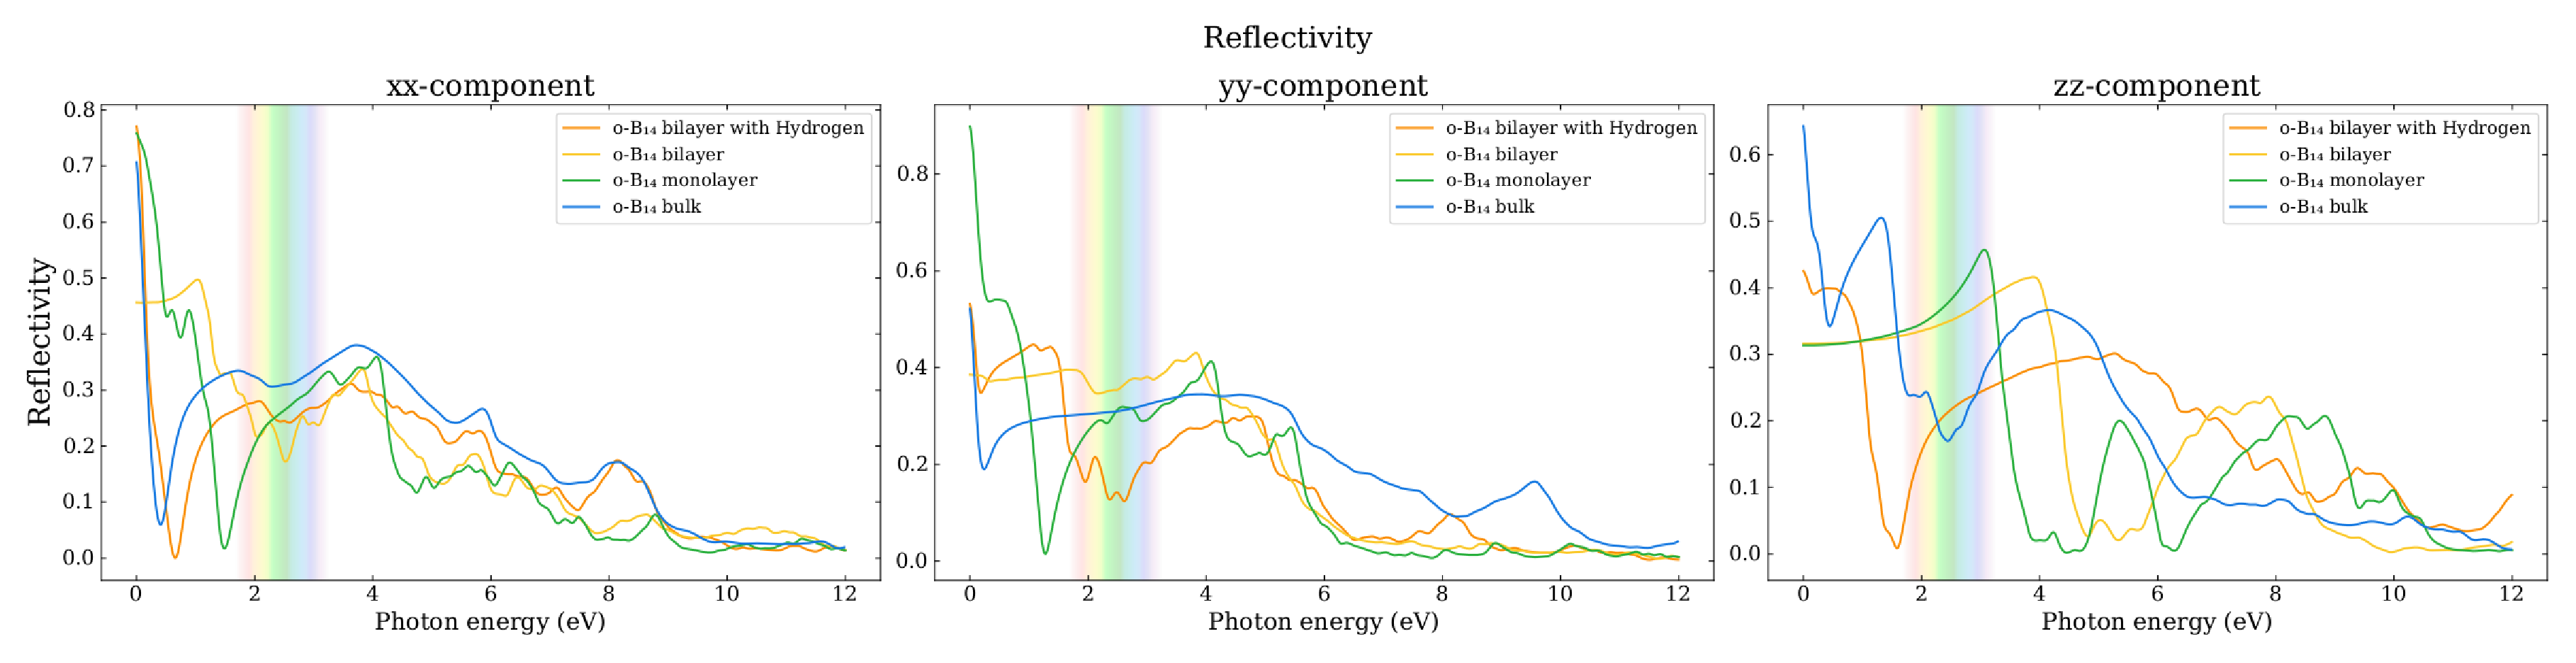
\includegraphics[width=1.0\linewidth]{fig-new-6.4_reflectivity.eps}
    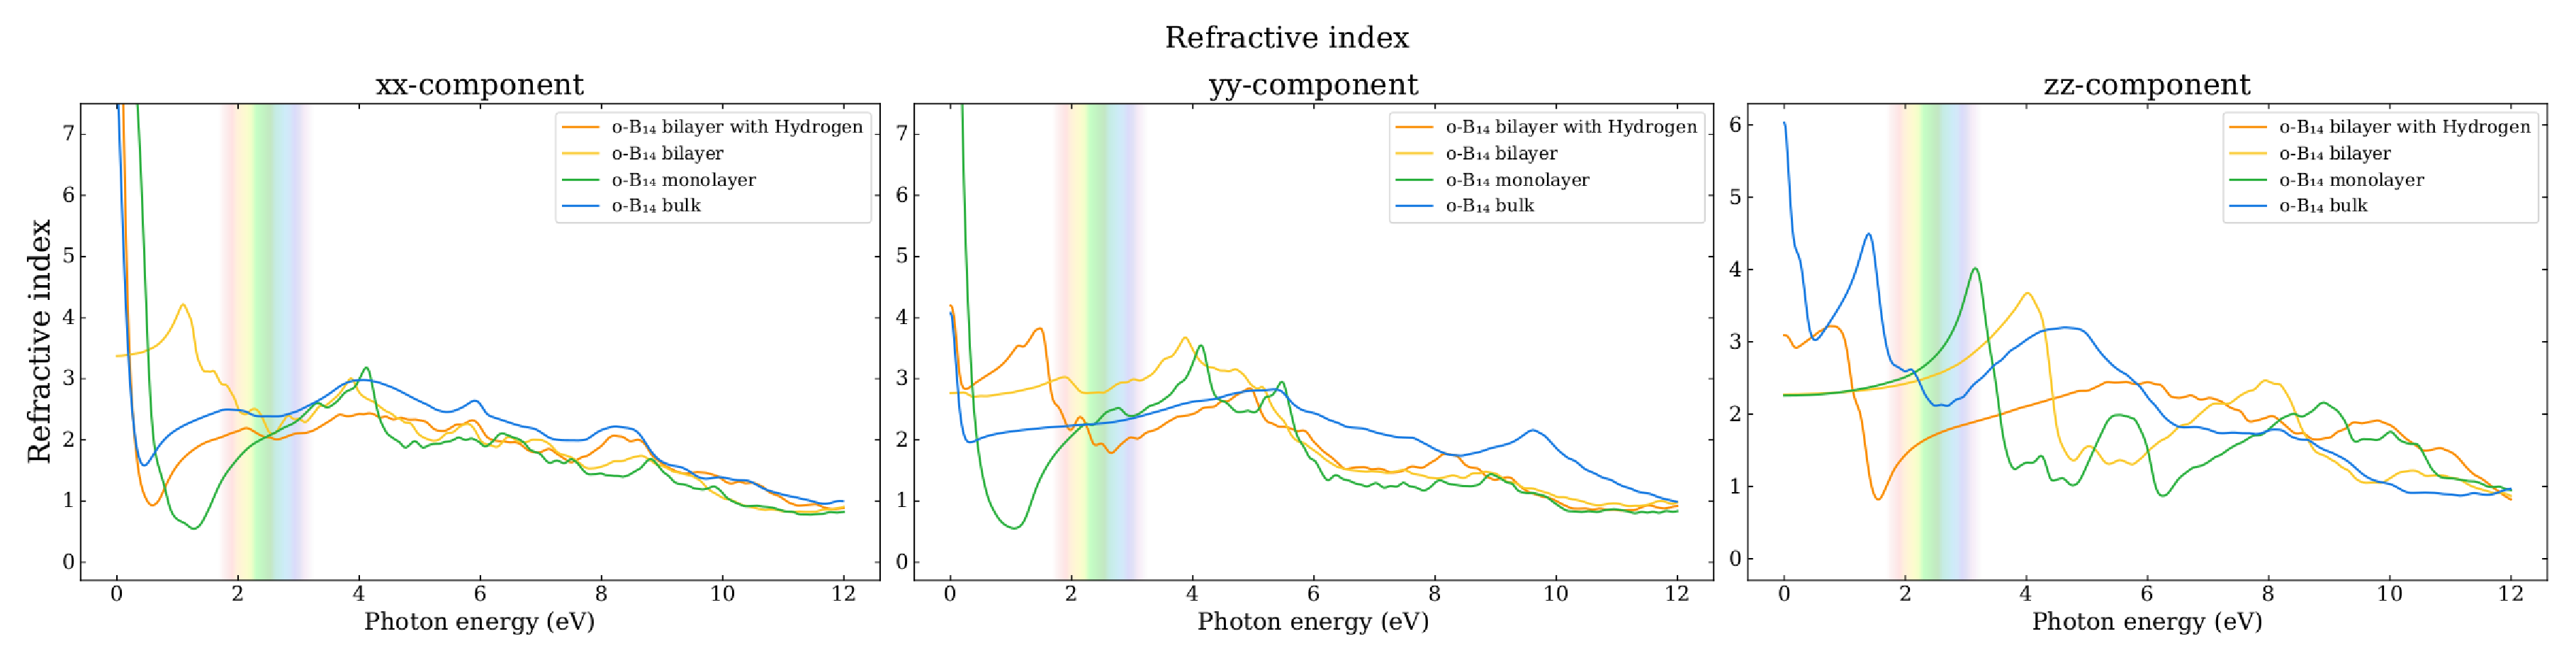
\includegraphics[width=1.0\linewidth]{fig-new-6.2_refractive.eps}
	\caption{The reflectivity and refractive index as a function of energy
	for the bulk and 2D o-B14 structures for the in-plane ($xx$, $yy$) and out-of-plane ($zz$) directions.}
    \label{fig-reflec-refrac}
\end{figure}
The extinction coefficient (imaginary part of the complex refractive index)
provides direct insight into how strongly a material absorbs light at different photon energies.
It is noticeable that
the extinction coefficient 
(shown in Fig.~S18) exhibits sharp dips near the above-mentioned plasmon 
resonances. Near a plasmon resonance, especially in surface plasmon
polaritons or localized surface plasmons, the dielectric function 
changes rapidly, both in the real and imaginary parts, and this affects
the extinction coefficient causing sharp features, including dips, 
near resonances. That is, these dips may indicate a frequency where 
the energy is lost not via absorption, but resonant energy transfer 
to the plasmon. Specifically, these dips are seen around (i) 0.5~eV and 1.3~eV 
($xx$),
1.0~eV and 6.0~eV ($yy$) and 3.5~eV and 6.0~eV ($zz$) for the monolayer; (ii) 2.0~eV ($yy$), 4.5~eV and 9.0~eV ($zz$) for the bilayer; (iii) 0.5~eV ($xx$), 2.0~eV and 6.0~eV ($yy$), and 1.5~eV ($zz$) for the H-bilayer; (iv) 0.5~eV and 
8.8~eV ($xx$), 0.2~eV and 10~eV ($yy$), and 0.5~eV, 2.0~eV and in the range 6.3-8.3~eV ($zz$) for the bulk.   
Overall, the plasmonic and optical properties of the o-B14 structures display 
interesting anisotropic effects that could offer 
opportunities for advanced optoelectronic, plasmonic  and quantum devices.



\section{Conclusion}

In the present work, the electronic, optical and superconducting properties of
novel o-B14 based structures were investigated on the basis of 
density functional theory calculations. Namely, we consider the three-dimensional
bulk as well as the 2D monolayer, bilayer, and 
hydrogen terminated bilayer. 
The cohesive energy of the monolayer is slightly less 
than that of the bulk (by 0.04~eV/atom), while the bilayer is notably more 
stable than the bulk (by 0.19~eV).
The 2D allotropes of o-B14 reveal complex properties including
semiconductivity in the bilayer (band-gap of 0.67~eV), 
magnetism in the monolayer 
and superconductivity in the hydrogen-terminated bilayer (with a $T_c$ of 24.3~K). 
The calculated optical properties show  absorption in the visible region 
of the spectrum for the bilayer, hydrogen terminated bilayer, and bulk in the $xx$, $yy$, and $zz$-directions, respectively.
All the metallic systems display plasmons in the in-plane direction for energies below around 1.5~eV, while plasmons are present for all systems in the out-of-plane direction. Interestingly, the monolayer and bulk 
systems behave as indefinite media, for which the real part of the dielectric
function in the in-plane and 
out-of-plane directions are of
opposite sign, namely in the region below 2.0~eV for the former, and 
between 6.0~eV and 10.0 eV for the latter, indicating directional 
plasmonic modes.
All together, these complex optical, electronic and superconducting 
properties emphasize the rich physics of boron materials which 
could hold potential for future high technologies. 



\section{Data Availability Statement}
The original data presented in the study are openly available in the 
GitHub repository 
Photonico/o-B14 20241024
at \url{https://github.com/Photonico/}.
\section{Acknowledgements}
This research was undertaken with the assistance of resources from the National Computational Infrastructure (NCI Australia), an NCRIS enabled capability supported by the Australian Government.
C.V. acknowledges financial support from the Australian Research Council 
(DE220101147) and 
C.S. acknowledges financial support from the Australian Research Council 
(FL230100176).

*Corresonding authors: Catherine Stampfl: catherine.stampfl@sydney.edu.au; Oliver Conquest: oliver.conquest@sydney.edu.au


\bibliographystyle{unsrt}
\bibliography{references.bib}

\end{document}
